\documentclass[12pt,spanish, singlespacing,]{MastersDoctoralThesis}
\usepackage[utf8]{inputenc} 
\usepackage[T1]{fontenc} 
\usepackage[none]{hyphenat}
\usepackage{palatino} 
\usepackage{acronym}
\usepackage{amsmath}
\usepackage{float}
\usepackage[caption = false]{subfig}
\spacing{1.5}
\usepackage[acronym,nomain]{glossaries}
%\usepackage[backend=bibtex,style=authoryear,natbib=true]{biblatex}
%\addbibresource{main.bib}
\usepackage[autostyle=true]{csquotes}
\usepackage{tikz}
\usetikzlibrary{shapes.geometric, arrows}
\usepackage{smartdiagram}
\usepackage{afterpage}
\tikzstyle{startstop} = [rectangle, rounded corners, minimum width=4cm, minimum height=1.5cm,text centered, draw=black, fill=blue!30]
\tikzstyle{arrow} = [thick,->,>=stealth]
\newcommand\blankpage{%
    \null
    \thispagestyle{empty}%
    \addtocounter{page}{0}%
    \newpage}
    
\usepackage{listings}
\renewcommand{\lstlistingname}{Código}
\renewcommand\lstlistlistingname{Índice de Código}

\usepackage{float}
\usepackage{url}
\makeatletter
\g@addto@macro{\UrlBreaks}{\UrlOrds}
\makeatother

\thesistitle{}
\supervisor{} 
\examiner{} 
\degree{} 
\author{} 
\subject{}
\keywords{} 
\university{\href{http://www.uni.edu.pe/}{Universidad Nacional de Ingenier\'ia}} 
\department{\href{http://fc.uni.edu.pe/fc/index.php/escuelas/ciencia-de-la-computacion}{}} 
\faculty{\href{http://fc.uni.edu.pe/fc/}{}}
\hypersetup{pdftitle=\ttitle} 
\hypersetup{pdfauthor=\authorname}
\hypersetup{pdfkeywords=\keywordnames} 
\sloppy
\decimalpoint
\begin{document}
\frontmatter 
\pagestyle{plain} 
\begin{titlepage}
\begin{center}
%\textsc{\huge \univname}\\[0.5cm]

\begin{figure}[h]
\centering

\includegraphics[width=0.3\textwidth]{Figures/log_uni.png}
\end{figure}

\textsc{\huge \univname}\\[0.3cm]
\textsc{\Large Facultad de Ciencias}\\[0.2cm]
\textsc{\large Escuela Profesional de Ciencia de la Computaci\'on}\\[2cm]
\textsc{\LARGE \textit{Métodos de optimización de la gradiente de descenso en una red neuronal convolucional}}\\[2cm] 
{\Large \textbf{SEMINARIO DE TESIS 1}}
{\huge \bfseries \ttitle}\\[2cm] 
% Thesis title
%\bigskip
%\HRule \\[0.8cm] % Horizontal line

%\begin{minipage}{1.5\textwidth}
%\begin{flushleft} \large
\bigskip
\bigskip
\large\emph{Autor: Víctor Jesús Sotelo Chico}
{\authorname}\\ 
\large\emph{Asesor: Víctor Melchor Espinoza}
{\supname} 
%\end{flushleft}
%\end{minipage}
%\\[2cm]
\\[1cm]
{\large Junio, 2018}\\[4cm] 
 
\vfill
\end{center}
\end{titlepage}
\afterpage{\blankpage}
%\cleardoublepage
%\renewcommand{\abstractname}{Abstract}
\begin{abstract}
\addchaptertocentry{\abstractname}
En las últimas décadas el campo de la inteligencia artificial se ha desarrollado rápidamente. Temas como el reconocimiento de imágenes han sido estudiado por mucho tiempo. Actualmente este campo requiere realizar un gran números de cálculos para entrenar redes neuronales que sean capaces de distinguir y clasificar distintos objetos contenidos en imágenes. Incluso este proceso puede tardar más dependiendo del tamaño del dataset. Por lo cual surge la necesidad de encontrar métodos que permitan acelerar el proceso de entrenamiento de las redes neuronales.\\
Por tal motivo presente seminario buscar lograr un mayor entendimiento de métodos para acelerar el proceso de entrenamiento de una red neuronal convolucional, basándonos en la teoría de redes neuronales y usando como herramienta la librería tensorflow, esta nos permite un uso controlado de las métodos de optimización.

\textbf{KEYWORDS}:  Dataset, Métodos Adaptativos, CNN, SGD, Optimizadores.
\end{abstract}\hspace{10pt}

\keywords{agasga}


\afterpage{\blankpage}
\tableofcontents
%\afterpage{\blankpage}
\listoffigures
%\afterpage{\blankpage}
%\listoftables
%\afterpage{\blankpage}
%\listoftables 
%\lstlistoflistings
%\afterpage{\blankpage}
\newpage

\begin{center}
{\huge Índice de Acrónimos}\\[2cm]
\end{center}
\bigskip
\begin{tabular}{ l c l }
\textbf{k-nn}& & k- nearest neighbors\\
\textbf{SVM}& & Super Vector Machine\\
\textbf{SVC}& & Super Vector Regression\\
\textbf{SVR}& & Super Vector Classification\\
\textbf{SGD} & & Stochastic gradient descent\\
\textbf{DNN} & & Deep Neural Network\\
\textbf{CNN} & & Convolutional Neural Network\\
\textbf{ETC} & & Etcétera \\

\end{tabular}
\afterpage{\blankpage}

\newpage
\begin{center}
{\huge \textit{Agradecimientos}}\\[1.5cm]
\end{center}

Agradezco a mis padres por todo el apoyo incondicional durante todos estos años de estudio, a mis compañeros de clase por el apoyo brindado durante el tiempo de estudio y a mi asesor por ayudarme en este seminario.



\afterpage{\blankpage}

\mainmatter 
\pagestyle{thesis}
\chapter{Introducción}
%-- 10 lineas
En el campo de la inteligencia artificial las redes neuronales profundas tienen un papel muy importante debido a que estas son el camino para que las computadoras realicen tareas que nuestros cerebros realizan de manera natural, tareas como el reconocimiento de voz, imagenes y patrones. En la actualidad empresas importantes utilizan las redes neuronales profundas uno ejemplo de esto es google con el reconocimiento de voz e imagenes. Un caracteristica de las redes neuronales profundas es que están compuestas por una gran cantidad de capas lo cual dificulta el entrenamiento en computadoras que solo usan el CPU. Una manera de resolver este problema es mediante el uso de las GPU's debido que las tareas de entrenamiento son paralelizables podemos usar las GPU'S para acelerar el proceso de entrenamientos de nuestra red neuronal profunda.

\section{Motivación}
La inteligencia artificial constituye una base muy importante en el campo de la computación, mezcla un conjunto de disciplinas como la estadística y ciencia de la computación con el objetivo de construir modelos que puedan permitir a las computadoras realizar tareas que hace años hubiese sido considerado imposible. El hecho de lograr que las computadoras sean capaces de reconocer objetos, clasificarlos lo cual ha permitido que la industria de la robotíca desarrolle de manera acelerada en las últimas décadas.  Hoy en día existen muchas herramientas que nos permiten desarrollar este tema y profundizarlo pero a medida que aumenta la complejidad del problema, el costo computacional incrementa lo cual se convierte un problema importante. Una de la soluciones que apareció fue el uso de la GPU's para acelerar procesos como el entrenamiento de una red neural con muchas capas ocultas, las GPU's representa una solución muy eficaz debido a que en el campo de la inteligencia artificial existen muchas tareas que son paralelizables. Actualmente el mercado de GPU's evoluciona muy rápido debido a su gran demanda en la industria de los videojuegos este mercado esta dominado por NVIDIA y AMD esta competencia y la alta demanda permite que las GPU's tengan mejor rendimiento, además actualmente la nube ofrece otra posibiliad para el desarrollo de GPGPU computing debido a que nos permite tener acceso a mejores recursos.

 Actualmente el uso de GPGPU computing es usado para acelerar los procesos ya que combina el uso de CPU's y GPU's 
%-----
%-----Que es lo que te ha motivado para realizar la tesis en esta temática y los aspectos más esenciales que pensabas obtener de ella...

%-----Este punto podrá ser de 4 páginas máximo. Es una de las partes más importantes que introduce al lector en el trabajo en tu tesis, por lo que debe estar muy bien redactado y estructurado.

\section{Objetivos}

El objetivo de este seminario es el de mostrar las ventanjas que presenta el uso de GPGPU computing frente a otro tipos de recursos en el entrenamiento de una deep neural network.

Especificamente, los objetivos de este trabajo con respecto al sistema son:

\begin{itemize}
\item[•] Entender el funcionamiento de las redes neuronales profundas%--OBJETIVO ESPECÍFICO 1.
\item[•] Mostrar los resultados de distintas GPU's en el entramiento de una red neuronal profunda.%--OBJETIVO ESPECÍFICO 2.
\item[•] Realizar un análisis comparar el rendimiento de cada GPU al momento de entrenar la deep neural network.%--OBJETIVO ESPECÍFICO 3.


\end{itemize}

Y los objetivos con respecto a las competencias académicas desplegadas en el trabajo son:
\begin{itemize}
\item[•] Desarrollar un manejo adecuado del uso GPU computing.%--OBJETIVO COMPETENCIA 1.
\item[•] Lograr un entendimiento de la tareas que son paralelizabeles en el entrenamiento de la red neuronal profunda.%--OBJETIVO COMPETENCIA 2.
\item[•] Desarrollar un manejo adecuado de tensorflow como herramienta para el reconocimiento de imagenes.%--OBJETIVO COMPETENCIA 3.

\end{itemize}

\section{Estructura del Seminario}


\begin{itemize}

\item \textbf{Introducción:} \\
En este capítulo introductorio se comentará sobres las motivaciones, objetivos con los cual se penso el presente seminario.
%--En este capítulo introductorio se comenta sobre las motivaciones ...

\item \textbf{Estado del Arte:} \\
En este capítulo observaremos los trabajos e investigaciones previa que tiene el presente seminario , además se expondrá el aporte que relizaremos.

%--\item \textbf{Metodología y Herramientas:} \\
%--....

%--\item \textbf{...} \\
%--Un pequeño texto más de ese capítulo(s) en concreto.

%--\item \textbf{Conclusiones y Trabajo a Futuro:}\\
%--En este capítulo se exponen las conclusiones obtenididas de este trabajo. Adicionalmente, se proponen trabajos a futuro para la implementación de el servidor y la aplicación web del sistema.
\end{itemize}

%--NOTA: RECUERDE QUE ES COMO UN LIBRO TODO CAPÍTULO NUEVO COMENZARÁ CON PÁGINA IMPAR NUNCA PAR



%\newpage
%$\ $
%\thispagestyle{empty} % para que no se numere esta pagina
\chapter{Estado del Arte}
En este capítulo se describirán las investigaciones anteriores con relación al Aprendizaje Automático, además de sus aplicaciones. También se verán algunas investigaciones referente al reconocimiento de voz y los algoritmos usados para estas tareas.

Este trabajo también presentará investigaciones referentes a Aprendizaje Profundo, exclusivamente nos enfocaremos a la Redes Neuronales Convolucionales(CNN), ya que son parte del tema de estudio en la presente investigación.

%---Escribir un texto de un o dos párrafo(s) máximo de 10 líneas con una introducción al capítulo 

%---El capítulo estado del arte es tanto o más importante que la tesis en sí. En el se debe especificar que desarrollo relacionado a tu tesis existe ya a nivel global y en que se diferencia tu trabajo de ellos. Por lo tanto un análisis exhaustivo de la especialidad y de los trabajos previos es tanto o más importante que el trabajo en sí, ya que indica un alto conocimiento de la materia si está bien estudiado.

%---En este capítulo van a ir muchas citas \cite{Wan09} de trabajos pero sobre todo de artículos científico, haga un buen estudio del arte \cite{Shuo10,Feldmann03}


\section{GPU computing}
Actualmente, el uso de GPU's permitió lograr aplicaciones que antes se podrían creer imposibles debido a su largo tiempo de ejecución. Hoy en día las GPUs son altamente usadas ya que cuentan con cientos de núcleos de procesadores en paralelo que permiten resolver rápidamente los problemas que son altamente paralelizables.
\subsection{The GPU computing Era}
	El artículo se enfoca principalmente en describir la evolución que sufrieron las arquitecturas de GPUs, además de mostrar la importancia del uso de las GPUs para un mayor rendimiento y eficiencia que antes hubiesen sido consideradas imposibles debido al alto tiempo de ejecución que requerían. Además nos muestra que la escalabilidad es la principal característica que ha permito que las GPUs aumenten su paralelismo y rendimiento.
\section{Aprendizaje Automático}
El uso del Aprendizaje Automático representa una gran ventaja para empresas que manejan gran cantidad de datos debido a que permiten descubrir patrones y analizar los datos.

\subsection{Uso de redes neuronales para encontrar el rendimiento de una GPU}
Un equipo conformado por investigadores \cite{GPU}de AMD y The University of Texas at Austin, fueron quienes propusieron el uso de redes neuronales para predecir el rendimiento de una GPU.
En la actualidad existen empresas dedicadas a la creación de GPUs, en el proceso una parte fundamental es la verificación del rendimiento de las GPUs. Actualmente existen simuladores conocidos como GPGPU-SIM que permiten realizar estimaciones precisas pero estos presentan algunas dificultades como el tiempo empleado en configurarlos en base al hardware real, no obstante, este proceso se encuentra propenso a errores. 
\subsection{Handshape recognition for Argentinian Sign	Language using ProbSom}
Investigadores de la Universidad de La Plata, en Argentina  conformado por Franco Ronchetti, Facundo Quiroga, César Estrebou, y Laura Lanzarini\cite{HAND}, desarrollaron un sistema que permite el reconocimiento de lenguaje de señas argentino. Esta investigación fue realizada usando una técnica llamada ProbSom, esta puede ser comparada con otros métodos como las Máquinas de Soporte Vectorial, Bosques Aleatorios y Redes Neuronales.
\section{Aprendizaje Profundo}
Dentro del área de Aprendizaje Automático encontramos Deep Learning o Aprendizaje Profundo el cual consiste en un conjunto de algoritmos que modela abstracciones de alto nivel.\\
En esta sección hablaremos de un paper que nos sirvió de un introducción al campo del aprendizaje profundo.

\subsection{Deep Machine Learning - A New Frontier in Artificial Intelligence}
Este trabajo de investigación fue realizado por investigadores Thomas	Karnowski, Derek Rose - Oak Ridge National Laboratory y Itamar	Arel - University of Tennessee \cite{DML}, el objetivo principal de este trabajo fue presentarnos el aprendizaje profundo como un camino para la imitación del cerebro humano y sus principales cualidades como el reconocimientos de objetos, rostros, etc.\\
En este paper presenta una introducción a los temas de \textit{Convolutional Neural Network(CNN)} y \textit{Deep Belief Network}, nos describe a las CNN como una familia de redes neuronales multicapas que fueron diseñadas para tratar datos de dimensionalidad 2 como lo son las imágenes y los videos.\\
Por otro lado, también nos muestra las aplicaciones del aprendizaje profundo como: análisis de documentos, detección de voz, rostro, procesamiento natural del lenguaje, etc.

La aplicación de la inteligencia artificial no solo despierto en los investigadores, también existen algunas empresas privadas que apoyan el campo del Aprendizaje Profundo con el objetivo de buscar sus aplicaciones comerciales, entre estas empresas tenemos a: Numenta y Binatix.
\section{Métodos de optimización}
El campo del Aprendizaje Automático continuamente evoluciona y con esta evolución surgen nuevas necesidades. Al trabajar con grandes conjuntos de datos se buscan cada vez obtener buenos resultados sin afectar el rendimiento. Una forma de lograr esto es mediante el uso de algoritmos de optimización.
\subsection{Neural Network Optimization Algorithms: A comparison study based on TensorFlow}
Vadim Smolyakov\cite{WEBSITE:11} realizo un estudio comparativo de diversos optimizadores entre los cuales se encuentran el método de gradiente de descenso estocástica, Nesterov Momentum, RMSProp y Adam. Se realizó una prueba comparativa con una arquitectura simple de CNN usando el conjunto de datos del MNIST. \textquotedblleft Se comparó diferentes optimizadores y se obtuvo que el SGD con Nesterov y Adam producen mejores resultados en el entrenamiento de una CNN simple usando tensorflow para el dataset MNIST. \textquotedblright \cite{WEBSITE:11}
\subsection{On Optimization Methods for Deep Learning}
Un equipo de la Universidad de Standford realizó unas pruebas con el objetivo de encontrar métodos adecuados para un entrenamiento en aprendizaje profundo. El equipo se percato de lo común que resulta el uso de gradiente de descenso estocástica (SGD por sus siglas en inglés) en aprendizaje profundo . Se realizaron pruebas con otros métodos de optimización como la gradiente conjugada y Limited memmory BFGS(L-BFGS) los cuales permitieron acelerar el proceso de entrenamiento de algoritmos de Aprendizaje Profundo mostrando en su mayoría mejores resultados que el SGD. \textquotedblleft Usando L-BFGS el modelo CNN alcanza el 0.69\%  en el estándar del MNIST dataset. \textquotedblright \cite{Optimization}

\subsection{Adam : A method for stochastic optimization}
Esta investigación fue la primera en plantear el método Adam para acelerar la gradiente de descenso. Fue propuesto por Diederik P. Kingma de la Universidad de Amsterdam y Jimmy Lei Ba de la Universidad de Toronto. Ellos describen el método Adam como un método sencillo de implementar, además que este utiliza pocos requisitos de memoria.
\textquotedblleft Nuestro método esta dirigido a problemas con grandes conjunto de datos y espacio de parámetros de alta dimensión. El método combina ventajas de otros métodos de optimización, la capacidad de Adagrad para manejar gradientes dispersos y la de RMSProp para tratar con objetivos no estacionarios\textquotedblright \cite{ADAM}
\vspace{2cm}
\subsection{Incorporating Nesterov Momentum into Adam}
Este trabajo fue realizado por Timothy Dozat de la Universidad de Stanford, en este paper se propone una mejora al método Adam modificando su componente de momento de esta manera se obtiene una convergencia más rápida.

\textquotedblleft Esencialmente la investigación muestra cómo combinar el momento clásico con una tasa de aprendizaje adaptativa. Este trabajo lleva un enfoque más allá de la investigación y mejora uno de los componentes principales sin aumentar la complejidad del algoritmo\textquotedblright \cite{NMIA}
\vspace{2cm}
\section{Reconocimiento de Voz}
\subsection{Review of Algorithms and Applications in Speech Recognition System}
Este trabajo fue realizado por CR Rashmi del \textit{ Cork Institute of Tecnology (CIT) } en la investigación se describe el reconocimiento del habla como un método poder realizar distintas aplicaciones como: reconocimiento del hablante(Identificación Biométrica), emociones, acento, etc. Además se presentan distintos algoritmos que usan transformada de fourier y modelos probabilísticos que son aplicados a tareas de reconocimiento de voz.\\ Esta investigación se centra en los algoritmos para la extracción de características y coincidencia de patrones.\\ Entre principales algoritmos para la extracción de características que muestran tenemos: RCC, MFCC, LPC, etc. Siendo el MFCC uno de los mejores para realizar tareas de reconocimiento del hablante. Por otro lado en coincidencia de patrones tenemos algoritmos como VQ, HMM, SVM, MLP, GMM, etc. Para tareas de reconocimiento de emociones y géneros destaca el GMM.

\section{Conclusiones}
%Hemos visto la necesidad....
A medida que tratamos muchos problemas vemos la necesidad de encontrar optimizadores adecuados para los diferentes tipos de problemas. En el área de Aprendizaje Profundo comúnmente se trabaja en el campo de reconocimiento de imágenes.\\ A pesar de las mejoras mediante el uso de GPUs este tipo de problemas necesitan soluciones óptimos para obtener un mejor rendimiento. Métodos como Nesterov Momemtum, RMSProp y Adam surgen como principales opciones para realizar optimizaciones de la gradiente de descenso.
%Poner unas conclusiones del capítulo y lo más importante, donde se enfoca tu trabajo y lo que se diferenncia del resto


%\newpage
$\ $
%\thispagestyle{empty} % para que no se numere esta pagina
\chapter{Machine Learning y Redes Neuronales}

En este capítulo trataremos los principales conocimientos de Aprendizaje automático como su clasificación y su importante dentro del campo de la inteligencia artificial, además exploraremos algunos modelos importantes. 
En este seminario se dará énfasis en los algoritmos de clasificación. Luego nos enfocaremos en las redes neuronales para tratar más a fondo los problemas de clasificación.

\section{Aprendizaje Automático}
Machine Learning o aprendizaje automático es una rama de la inteligencia artificial que empezó a cobrar cobrar importancia en los años 80's, en esta rama se diseñan sistemas que aprenden a identificar patrones en un conjunto de datos. A medida que se realice este aprendizaje la máquina podrá ser capaz de realizar una predicción o tomar decisiones sin haber estado programada explícitamente para realizar esta tarea.


El aprendizaje automático se puede clasificar en 3 tipos: Supervizado, No supervisado, Aprendizaje con refuerzo.\cite{WEBSITE:2}
\subsection{Aprendizaje Supervizado}
Este tipo de aprendizaje  toma un conjuto de datos etiquetados, es decir datos cuyos resultados o clases son conocidos estos datos serán usados como entrada al sistema. Primero se entrena el modelo con los datos de entrada y luego se trata de predecir  una salida de acuerdo a sus etiquetas.

 \textquotedblleft El aprendizaje supervisado trata de modelar la relación entre el resultado de la predicción y las características de las entradas de manera que se puede predecir nuevos valores para un nuevo conjunto de datos \textquotedblright \cite{WEBSITE:1}
\subsection*{Tipos de problemas}
Dentro del aprendizaje supervisado podemos dividir los problemas en 2 tipos:
\subsubsection*{Problemas de Regresión Lineal}
Los problemas de regresión lineal son muy conocidos en el ámbito de aprendizaje automático y la estadística 
\subsubsection*{Problemas de Clasificación}
\textquotedblleft En este tipo de problemas se predice una respuesta del tipo categórica de manera que se puedan separar los datos mediante clases. \textquotedblright \cite{WEBSITE:2}

\textquotedblleft El objetivo de los problemas de clasificación es asignar las observaciones en categorías discretas en lugar de estimar valores continuos. \textquotedblright \cite{WEBSITE:1}


\begin{figure}[H]
	\centering
	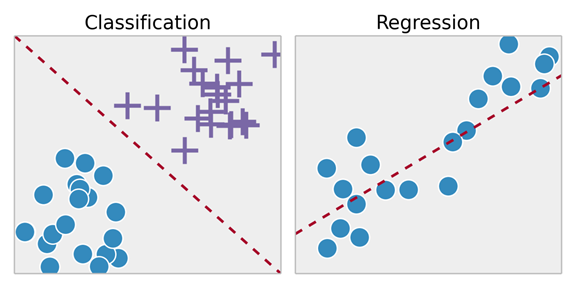
\includegraphics[width=0.9\textwidth]{Figures/regreclas.png}
	\caption{Regresión y clasificación \\ Fuente:  \href{https://medium.com/deep-math-machine-learning-ai/different-types-of-machine-learning-and-their-types-34760b9128a2}{\textit{https://medium.com/}}}
	\label{Regresion}
\end{figure} 

\subsubsection*{Algoritmos de Aprendizaje Supervizado}
\subsubsection*{Regresión Lineal}
\textquotedblleft El algoritmo de regresión lineal asume que existe una relación entre las variables de entrada $x=(x_{1},...,x_{n})$ y una salida simple $y$.  Cuando se tiene solo una variable simple $x$ el método se conoce como simple linear regression y cuando se tienen múltiples entradas se le conoce como multiple linear regression.  \textquotedblright \cite{WEBSITE:3} .Es comúnmente usado para estimar valores reales en base a variables continuas. La figura 3.2 muestra una regresión lineal simple.
\begin{equation}
\label{Simple learning regression}
y=b_{0}+b_{1}*x_{1}+b_{2}*x_{2}+.....+b_{n}*x_{n}
\end{equation} 
En esta ecuación:
\begin{itemize}
	\item $y$    : Variable dependiente
	\item $x_{i}$: Variable independiente i
	\item $b_{0}$: Intercepción
	\item $b_{1}$: Coeficiente para la primera característica
	\item $b_{n}$: Coeficiente para la primera característica
	
\end{itemize}
El objetivo del algoritmo de regresión lineal es obtener valores adecuados para $b_{0}$ y $b_{1}$ de manera que se reduzca la siguiente función de costo.
 \begin{equation}
 \label{eq:T3}
 \begin{aligned}
 J&=\frac{1}{n} \sum_{i=1}^{n}(pred_{i}-y_{i})^2
 \end{aligned}
 \end{equation}


\begin{itemize}
	\item $pred_{i}$: predicción de la i-esima variable
	\item $y_{i}$   : Valor real asociado a la i-esima variable
	\item $n$       : Número de datos para el entrenamiento
	
\end{itemize}
Un método muy importante es la gradiente de descenso que se usa para actualizar los valores de los $b_{i}$ de manera que se reduzca la función de costo $J$ de la ecuación 3.2.
\begin{figure}[H]
	\centering
	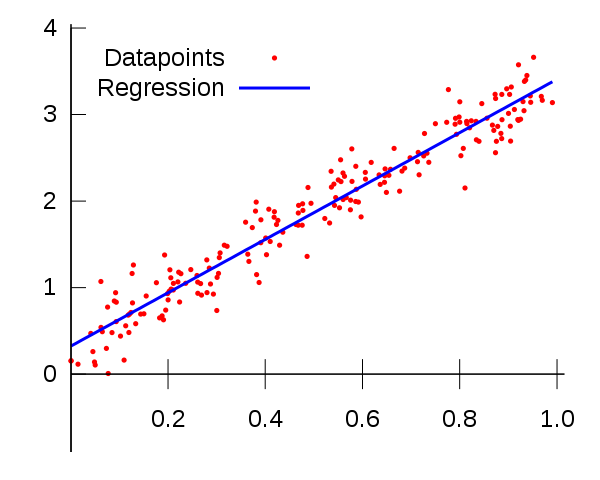
\includegraphics[width=0.9\textwidth]{Figures/Linear.png}
	\caption{Regresión Lineal \\ Fuente:  \href{https://www.forexmt4indicators.com/linear-regression-mt4-indicator/}{\textit{www.forexmt4indicators.com/}}}
	\label{Regresión Lineal}
\end{figure} 

\subsubsection*{Regresión Logística}
A diferencia de la regresión Lineal, la regresión Logística es usado para precedir el resultado de un variable de tipo categórica es decir variables que pueden ser describen por un número finito de categorías.

 La regresión Logística es usado para problemas de clasificación lo hace mediante la predicción de que una salida $Y$ sea dicotoma es decir que solo tenga 2 posibles valores.
 la regresión produce una curva la cual produce valores entre 0 y 1.
 \textquotedblleft Matemáticamente podemos como que las salidas están modeladas como una combinación de los predictores lineales.\textquotedblright \cite{WEBSITE:6}
 \begin{equation}
 \label{eq:t}
 \begin{aligned}
 odds &= p/ (1-p)\\ 
 ln(odds) &= ln(p/(1-p))\\      
 logit(p) &= ln(p/(1-p)) = b_{0}+b_{1}X_{1}+b_{2}X_{2}+b_{3}X_{3}....+b_{k}X_{k}
 \end{aligned}
 \end{equation}
 %\end{equation} 
 
 \begin{itemize}
 	\item p : probabilidad de presencia de una característica de interés.
 	\item odds: probabilidad de éxito.
 	\item logit: función logit
 \end{itemize}
 
 Despejando p de las ecuaciones anteriores de 3.2 podemos obtener que:
  \begin{equation}
  \label{eq:t1}
  \begin{aligned}
  p&=\frac{1}{1+e^{b_{0}+b_{1}X_{1}+b_{2}X_{2}+b_{3}X_{3}....+b_{k}X_{k}}} \\
  Y_{pre}&=\frac{1}{1+e^{f(X)}}
  \end{aligned}
  \end{equation}
 En la ecuación 3.3, $Y$ define la función logística que se muestra en la figura 3.3. Esta forma también se puede conocer como la función sigmoidal en el perceptron.
 El algoritmo usa SGD para hallar los valores adecuados de $b_{i}$ de manera que el $erro=Y_{pre}- Y$ sea mínimo.
 El valor de la predicción es 1 si $Y_{pred}>0.5$ y 0 en caso contrario. De esta forma se determina el objeto con características $X$ si pertenece o no a una clase.
 
 \begin{figure}[H]
 	\centering
 	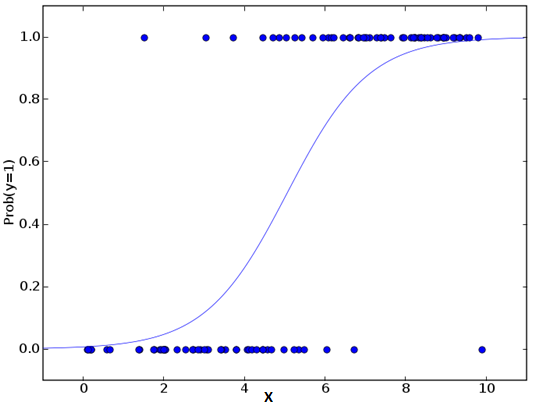
\includegraphics[width=0.9\textwidth]{Figures/logistic.png}
 	\caption{Regresión Logística \\ Fuente:  \href{https://www.analyticsvidhya.com/blog/2017/09/common-machine-learning-algorithms/}{\textit{www.analyticsvidhya.com}}}
 	\label{Regresión Logistica}
 \end{figure} 
\subsubsection*{Nearest Neighbor}
Es un algoritmo de clasificación que almacena los conjuntos de entrenamiento de manera que dado un nuevo ejemplo $x$ lo clasifica buscando la distancia  más cercana a un ejemplo de entrenamiento $(x_{i},y_{i})$ de manera que identifica la clase $y=y_{i}$ a la que corresponde.

 Comúnmente se usa el algoritmo k-nn para clasificar una entrada $x$ en los k más cercanos conjuntos de entrenamiento y asigna el objeto a la clase de más frecuencia.

  \begin{equation}
  \label{eq:t12}
  \begin{aligned}
  x^i=(x_{1}^i,x_{2}^i,.... ,x_{n}^i)\\
  d_{E}(x^i,x^j)
  \end{aligned}
  \end{equation}
\begin{itemize}
	\item $x^i$: objeto con n características.
	
\end{itemize}

Definimos $d_{E}$ como la función distancia entre los vectores  $x_{i}$ y $y_{i}$ están función distancia pueden una de las siguientes clasificaciones:

  \begin{itemize}

  \item distancia euclideana:    $(\sum_{i=1}^{k}(x_{i} - y_{i})^2)^\frac{1}{2}$
  \item distancia Manhattan:     $\sum_{i=1}^{k}|x_{i} - y_{i})|  $
  \item distancia Minkowski:     $(\sum_{i=1}^{k}(|x_{i} - y_{i}|)^p)\frac{1}{p}$
  \end{itemize}
Los 3 definiciones anteriores de distancia son usadas para variables continuas.  Para el caso de variables categóricas debería usarse la distancia de Hamming cuya definición se muestra en la ecuación 3.6


  \begin{equation}
  \label{eq:t6}
  \begin{aligned}
  	D_{H}&=\sum_{i=1}^{k}|x_{i} - y_{i})|\\
  	x&=y \Longrightarrow D=0\\
  	x&\neq y \Longrightarrow D=1
  \end{aligned}
  \end{equation}
  	
\textquotedblleft La elección de un valor óptimo de k se logra mejor por la inspección de los datos. En general un valor grande de k es más preciso ya que reduce el ruido pero no hay garantías de que sea un valor correcto, una mejor manera de calcular el valor de $k$ es mediante el uso de la validación cruzada.
\textquotedblright \cite{WEBSITE:7}

En la figurar 3.4 muestra el algoritmo de k-nn dado un nuevo ejemplo(círculo verde) este será clasificado a de acuerdo seleccionado. Para $k=1$ el nuevo ejemplo será clasificado en la clase 1 y $k=3$ será clasificado en la clase 2.
 \begin{figure}[H]
 	\centering
 	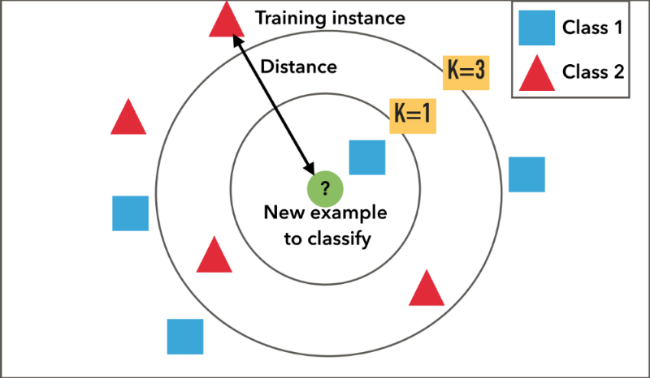
\includegraphics[width=0.7\textwidth]{Figures/knn.png}
 	\caption{knn \\ Fuente:  \href{https://medium.com/@adi.bronshtein/a-quick-introduction-to-k-nearest-neighbors-algorithm-62214cea29c7}{\textit{www.medium.com/}}}
 	\label{knn}
 \end{figure} 
\subsubsection*{Máquinas de soporte Vectorial(SVM)}
Las Maquinas de soporte vectorial fueron creadas por Vladimir Vapnik y constituyen un método para realizar tareas de clasificación y regresión.\\ Las SVM usan el concepto de planos de decisión. Un plano de decisión separa un conjunto de objetos que tienes diferentes etiquetas de clases. Las SVM no están restringidas a los problemas lineales debido a las \textit{funciones Kernel.}
\textbf{Funciones Kernels}\\
Las SVM pueden tener distintos tipos de kernels que tienen como objetivo tomar la data y transforma una forma requerida algunas de estas funciones son:
\begin{itemize}
	\item Lineal: $\ker(x_{i},x_{j})= x_{i} \cdot x_{j}$
	\item Polinomial: $\ker(x_{i},x_{j})= ( \gamma x_{i} \cdot x_{j}+C)^d$
	\item Radial: $\ker(x_{i},x_{j})= e^{(\gamma |x_{i} - x_{j}|)}$
	\item Sigmoidal: $\ker(x_{i},x_{j})= \tanh ( \gamma x_{i} \cdot x_{j}+C)$
\end{itemize}
En la figura 3.5 muestra el efecto de las funciones kernels en un conjunto de datos para que este sea linealmente separable sin necesidad de construir curvas complejas.\\
\begin{figure}[H]
	\centering
	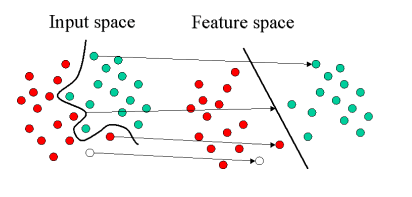
\includegraphics[width=0.9\textwidth]{Figures/kernel.png}
	\caption{transformación con la función kernel \\ Fuente:  \href{http://www.statsoft.com/Textbook/Support-Vector-Machines}{\textit{www.statsoft.com}}}
	\label{transformación con la función kernel}
\end{figure} 

Podemos dividir SVM en 2 categoríasas:\\
\textbf{Super Vector Classificacion}\\
Los SVC realizan la tarea de clasificación encontrando un hiperplano que maximeze el margen entre 2 clases.Los vectores que definen el hiperplano son llamados \textit{support vector}.\\ Para la clasificación es necesaria mapear los datos a un espacio de características de mayor dimensión donde resulte más fácil la separación lineal.  La imagen de la Figura 3.5 muestra de manera gráfica que cambio de espacio nos permite separar clases de manera más sencilla.\\ \\
\textbf{Super Vector Regression}\\
La idea de SVR trata de mapear los datos de entrenamiento $x \in X$ , a un espacio de mayor dimensión mediante una mapeo no lineal $ \varphi : X \to F$ .\\
Las SVR son parecidas a las máquinas de soporte Vectorial para la clasificación pero con la diferencia de que la salida es un número real que es difícil de predecir con la información que se posee además de que tiene infinitas posibilidades. Para los problemas de regresión se usan los kernels Radial y polinomial. La figura 3.6 muestra un ejemplo de problema de regresión para un caso no lineal, mediante la mapeo $ \varphi $ se cambia el espacio.

\begin{itemize}
	\item caso lineal:     $y=\sum_{i=1}^{N}(\alpha_{i}  -\alpha_{i}^*)\langle x_{i},x\rangle +b$
	\item caso no lineal:  $ y=\sum_{i=1}^{N}(\alpha_{i}  -\alpha_{i}^*)\ker(x_{i},x) +b$
\end{itemize}

\begin{figure}[H]
	\centering
	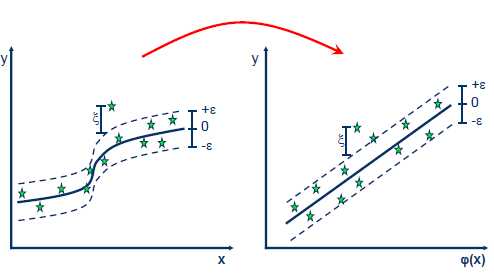
\includegraphics[width=0.7\textwidth]{Figures/SVR.png}
	\caption{transformación para un problema de regresión \\ Fuente:  \href{http://www.saedsayad.com/support_vector_machine_reg.htm}{\textit{www.saedsayad.com}}}
	\label{transformacion}
\end{figure} 

\subsubsection*{Naive Bayes}
Esta basado en el teorema de bayes donde se asume la independencia entre los predictores.
Es una técnica de clasificación basada en el teorema de bayes suponiendo que las características de una clase no esta relacionada con otra característica un ejemplo de esto es \textquotedblleft una fruta puede considerarse una manzana si es roja, redonda y de aproximadamente 3 pulgadas de diámetro. Incluso si estas características dependen unas de otras o de la existencia de otras características, todas estas propiedades contribuyen de forma independiente a la probabilidad de que esta fruta sea una manzana y es por eso que se la conoce como \textbf{naives}  \textquotedblright \cite{WEBSITE:4}
\subsubsection*{Decision Trees}
El árbol de decisión construye un modelo basado en los actuales valores de los datos. La decisiones se difurcan en la estructura de árbol hasta que se toma una decisión de predicción para un registro dado. Los arboles de decisión están entrenada para problemas de clasificación y regresión . Una de las principales ventajas de los arboles de decisión es que son rápidos y precisos.
\subsubsection*{Neural Networks}
Los modelos de redes neuronales fue inspirado de las redes neuronales biológicas y realizan tareas complejas como reconocimiento de imágenes
El tema de Neural Network será tratado con más detenimiento en el capítulo 4.
\subsection{Aprendizaje No Supervizado}
Mientras que el aprendizaje supervizado aprende  de un conjunto de datos de entrenamiento con respuestas o etiquetas correctas. En el aprendizaje no supervizado los datos de entrenamiento no poseen ninguno tipo de etiqueta, el sistema debe de interpretar los datos por si mismo.
El aprendizaje no supervizado es usado principalmente para el reconocimiento de patrones y modelado descriptivo.
\subsubsection*{Clustering}
Clustering se refiere a agrupar objetos con características similares es decir se busca la relación entre ellos sin necesidad de que exista un conocimiento a priori de esos grupos.
\begin{figure}[H]
	\centering
	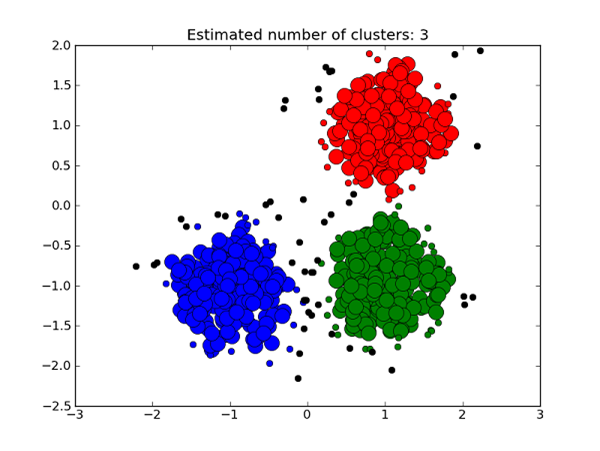
\includegraphics[width=0.9\textwidth]{Figures/clustering.png}
	\caption{Clustering \\ Fuente:  \href{https://medium.com/deep-math-machine-learning-ai/different-types-of-machine-learning-and-their-types-34760b9128a2}{\textit{https://medium.com/}}}
	\label{Clustering}
\end{figure} 
\subsubsection*{K-means Clustering}
el algoritmo
\subsection{Aprendizaje por refuerzo}
Este tipo de aprendizaje fue inspirado por la psicología conductista, este tipo busca determinar que tipo de acciones tomar en un entorno dado. \textquotedblleft El objetivo del método es recopilar la interacción con el entorno para tomar acciones que maximicen el beneficio o minimicen el riesgo. \textquotedblright \cite{WEBSITE:1}
\begin{figure}[H]
	\centering
	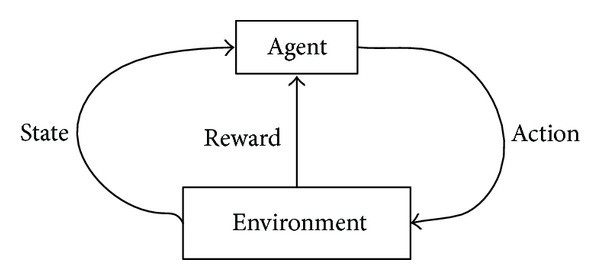
\includegraphics[width=0.9\textwidth]{Figures/esquema.jpeg}
	\caption{Esquema de aprendizaje por refuerzo \\ Fuente:  \href{https://towardsdatascience.com/types-of-machine-learning-algorithms-you-should-know-953a08248861}{\textit{https://towardsdatascience.com}}}
	\label{refuerzo}
\end{figure} 


\section{Redes Neuronales}
\subsection*{Neuronas}
En la biología la neurona es conocida como la unidad fundamental del cerebro humano, el cual está compuesto por millones de neuronas interconectadas entre si. El trabajo de las neuronas consiste en recibir información, procesarla y enviarla a otras células. Este modelo fue copiado en 1943 por Warren S. McCulloch y Walter H. Pitts. Analogamente con las neuronas del cerebro humano nuestra neuro artificial toma una cantidad n de entradas $x_{1}, x_{2}, x_{3}, .. , x_{n}$ estas entradas serán multiplicadas por pesos $w_{1}, w_{2}, w_{3}, .. , w_{n}$ además se puede añadir una constante que llamaremos bias. 

La entrada a de la neurona será la suma total de los productos z=  $\sum_{i=1}^{n}x_{i}$ , el valor de z será la entrada a la neurona la cual la evaluará con una función f de tal forma que nuestra salida sea $y=f(z)$. Otra forma de ver esta expresión es por medio de la notación de vectores donde representaremos a las entradas como $x= [x_{1}  x_{2}  x_{3}  ...  x_{n}]$ y los pesos w= $[w_{1}  w_{2}  w_{3}  ...  w_{n}]$ de esta manera la salida de la neurona estará dada por $y=f(x\cdot w+b)$ donde b representa las bias. 

\subsection*{Redes Neuronales Artificiales}
Las redes neuronales artificiales(ANN)toman de ejemplo la arquitectura del cerebro como inspiración para la construcción de sistemas inteligente. Actualmente son la base para el desarrollo de la inteligencia artificial. Las redes neuronales están constituidas de las uniones de las neuronas. 
\subsection*{Redes Neuronales Profundas}


Las redes neuronales profundas estan constituidas principalmente de un numero de capas de convolución, No linearalidad y pooling.
\begin{itemize}
	\item Convolución:
	Un proceso importante dentro de las redes neuronales es la convolución que es usada para detectar las características de una imagen estas características pueden ser bordes, curvas, etc.
	\item No linearalidad:
	Debido a que las convoluciones son operaciones lineales, lo cual no es adecuado para las tareas del mundo real. Debido a esto es importante introducir el ReLu que aplicará funciones no lineales a los mapas de característica producidas en las capas de convolución.
	Una de las funciones las común es ReLu.
	\begin{figure}[H]
		\centering
		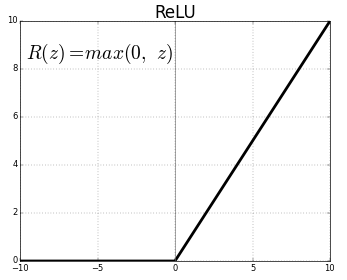
\includegraphics[width=0.5\textwidth]{Figures/relu.png}
		\caption{ReLu  Fuente:
			\href{https://medium.com/@kanchansarkar/relu-not-a-differentiable-function-why-used-in-gradient-based-optimization-7fef3a4cecec}{\textit{https://medium.com/}}
			 }
		\label{ReLu}
	\end{figure}

	
	\item Pooling:
	Sirve para transformar el mapa de características en una representación de menor dimensión con el objetivo de la red sea más invariante a pequeñas transformaciones o variación de la imagen de entrada.
\end{itemize}



%%\subsubsection*{Características}
%%%
%%\begin{figure}[H]
%%\centering
%%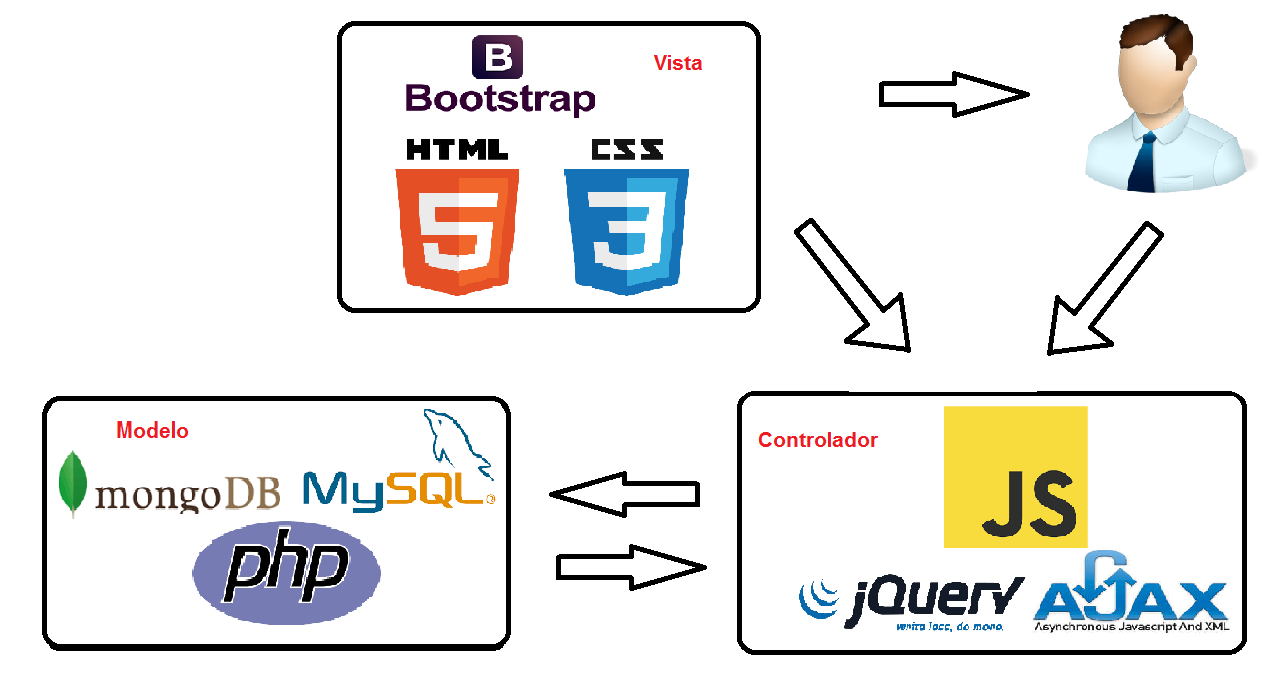
\includegraphics[width=0.9\textwidth]{Figures/mvc.png}
%%\caption{Modelo-Vista-Conrolador}
%%\label{MVC}
%%\end{figure}



\afterpage{\blankpage}
%\newpage
$\ $
%\thispagestyle{empty} % para que no se numere esta pagina
\chapter{Optimizadores para la gradiente de descenso en una Red Neuronal Convolucional}
En este capítulo se detallarán algunos algoritmos de optimización de Aprendizaje automático y principalmente se enfocará en aquellos que serán utilizados en nuestra red neuronal convolucional.\\
Al inicio de este capítulo veremos una introducción a este tipo de redes de prealimentación.

\section{Redes Neuronales Convolucionales}
Las CNN son un tipo de redes neuronales especiales para procesar datos como imágenes las cuales son más difíciles de tratar en una red neuronal tradicional, como por ejemplo en el caso del perceptron multicapas.\\ El término \textit{convolucional} hace referencia a la operación lineal matemática usada. Las redes neuronales convolucionales usan esta operación para aprender de las características de mayor orden presente en los datos.
La primera CNN fue creada por Yann LeCun. Entre sus usos más comunes tenemos el reconocimiento de imágenes y lenguaje natural.\\
Las redes neuronales convolucionales fueron inspiradas en la corteza visuales de los animales. Las células de la corteza visual, estas se activan para realizar tareas como el reconocimiento de patrones.

\subsection{Estructura de una imagen}
Debido a que las redes neuronales convolucionales trabajan principalmente con imágenes, es importante conocer cual es la estructura de una imagen y cómo es que la computadora comprende y utiliza esta información.\\
Las imágenes están constituidas por una sucesión de píxeles, podemos entender el pixel como la menor unidad homogénea en color de una imagen digital. Teniendo este concepto, podemos dividir la información de una imagen de la siguiente forma:
\begin{itemize}
	\item \textbf{Width}: El ancho de la imagen medido en pixeles
	\item \textbf{Height}: El alto de la imagen medida en pixeles.
	\item \textbf{Canales RGB}: Estos canales contiene la información de los colores y profundidad de una imagen. Este canal guarda la información en tres canales Red, Green y Blue.
\end{itemize}

\begin{figure}[H]
	\centering
	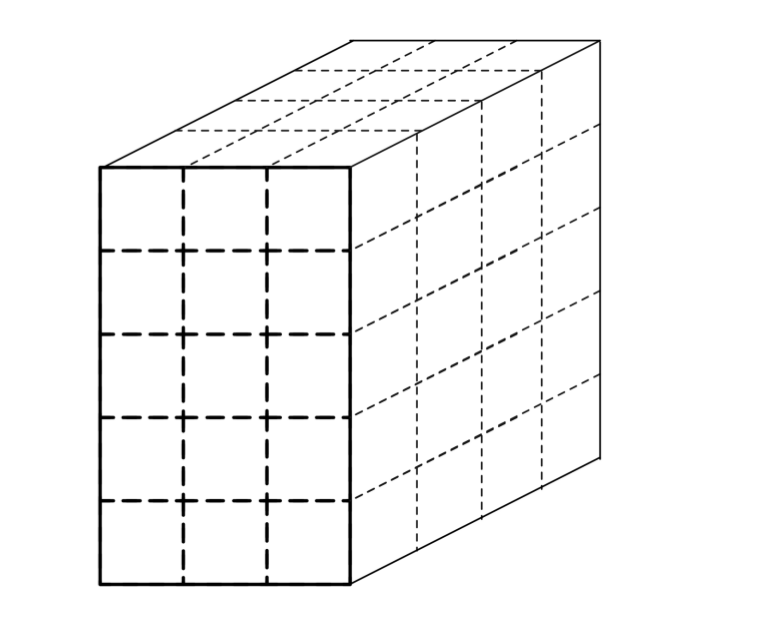
\includegraphics[width=0.7\textwidth]{Figures/image.png}
	\caption{Estructura de la imagen de entrada \\ Fuente:  \href{https://www.safaribooksonline.com/library/view/deep-learning/9781491924570/ch04.html}{\textit{Deep Learning by Adam Gibson, Josh Patterson}}}
	\label{image}
\end{figure} 

Teniendo en cuenta esta forma de guardar una podemos resaltar la ventaja de usar Redes convolucionales en lugar de usar una red neuronal multicapas.\\ Las redes multicapas toman un vector de una dimensión como entrada, si quisiéramos entrenar un perceptron multicapas con imágenes de 32x32 píxeles y con 3 canales RGB necesitaríamos crear 3072 pesos ($w_{i}$) para una sola neurona en la capa oculta. Esta generación excesiva de peso hace que la tarea resulte complicada usando redes multicapas.\\ De esta forma surge la idea de recurrir a un tiempo tipo de redes neuronales que faciliten la tarea sin consumir muchos recursos.
\subsection{Capas de una CNN}
Las redes neuronales convoluciones pueden ser dividas en distintas capas, cada una con una tarea específica para el tratamiento de la información. En esta sección describiremos cada una de estas capas.
\subsubsection{Input layer}
Esta capa es la encargada de cargar y almacenar la información de las imágenes para luego procesarlas en la red. Esta información contiene detalles de ancho, alto en píxeles y el número de canales de imagen. Las entradas de esta capa corresponden a la imagen vista en la figura 4.1.

\subsubsection{Convolutional layers}
Es una de las capas más importante en el diseño de las CNNs, esta capa es la encargada de transformar la entrada(imagen o convolución anterior) usando las conexiones de las neuronas en capas anteriores. La capa calculará el producto punto entre la región de las neuronas de la capa de entrada y los pesos a los que están colocados localmente en la capa de salida. Esta salida tendrá la misma dimensión de espacios o una dimensión menor.

Para entender más a fondo esta capa debemos definir la operación de \textit{convolución}.  La \textit{convolución} es una operación matemática que describe una regla de como fusionar 2 conjuntos de información.\textquotedblleft Esta operación tiene importancia en campos como la matemática y la física debido que permite definir un puente entre el domino del espacio/tiempo y el dominio de la frecuencias a través del uso de la transformada de fourier.\\
La convolución toma la entrada, aplica un kernel de convolución y nos da un mapa de características como salida \textquotedblright \cite{book1} .\\
Las convoluciones son usadas principalmente como un detectores de características cuyas entradas son la capa de entrada u otra convolución.
En la figura 4.2 observamos la operación de convolución que por medio del uso de un kernel o filtro de convolución extrae características de la imagen, por ejemplo detalles como bordes de una imagen.\\ Haciendo analogía con los pesos en las redes neuronales convencionales, las redes poseen el \textit{ filtro o kernel }, esto resulta beneficioso, ya que no se tendrá definir un peso para cada neurona.\\ En la figura 4.2 vemos como se aplica el kernel para producir datos de característica, este kernel será desplazado a lo largo de las dimensiones espaciales. En el desplazamiento el kernel se multiplicará por los datos de entrada dentro de su limite, produciendo una sola salida al mapa de características.
\begin{figure}[H]
	\centering
	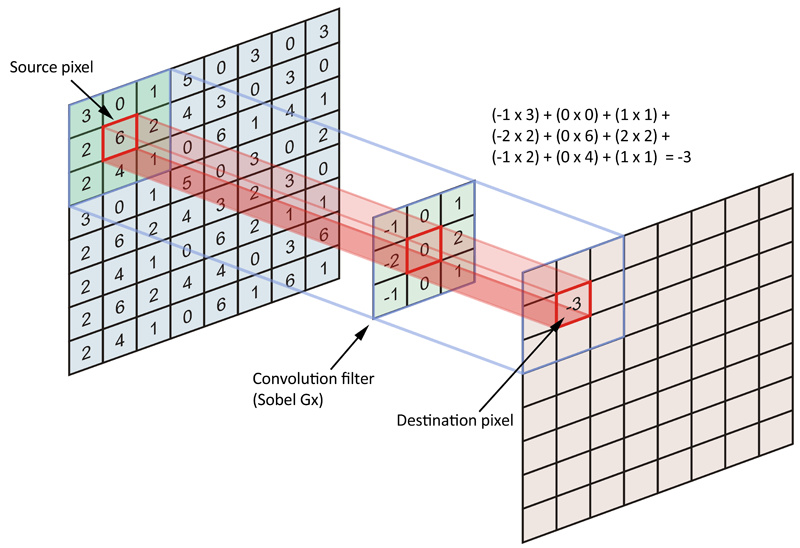
\includegraphics[width=0.7\textwidth]{Figures/convolucion.jpeg}
	\caption{Operacion de convolución \\ Fuente:  \href{http://openresearch.ai/t/network-in-network/39}{\textit{www.openresearch.ai}}}
	\label{convolucion}
\end{figure} 

Las capas convolucionales aplican transformaciones o funciones de activación al conjunto de entrada, luego el mapa de activación generado se apilará a lo largo de dimensión de profundidad para construir el volumen de salida.

\textbf{Componentes de la capa de convolución}.\\	
Las capas convolucionales poseen parámetros e hiperparámetros. La gradiente de descenso tiene la funcion de entrenar los parámetros de modo que las clases sean consistentes con las etiquetas en el conjunto de entrenamiento. Entre estos parámetros tenemos:
\textbf{Filtros}

Los filtros son una función que posee ancho(width) y alto (height) más pequeños que la entrada. Los filtros son aplicados a través de  del ancho y alto de la entrada, pero también pueden ser aplicados a lo largo de la profundidad.

\textbf{Hiperparámetros de una capa de convolución}.\\
A continuación veremos algunos hiperparámetros que determinan la disposición espacial y tamaño del volumen de salida de una capa convolucional.
\begin{itemize}
	\item \textbf{Filter size:} Cada filtro es pequeño con respecto al ancho(width) y alto(height) del la capa anterior. Por ejemplo podemos tener un filtro de tamaño $[5x5x3]$, lo representa 5 de ancho x 5 de alto x 3 de los canales RGB.
	\item \textbf{Output depth:} Este hiperparámetro controla el número de neuronas en la capa convolucional que están conectadas al mismo del volumen de entrada. Este parámetro puede ser elegido manualmente.
	\item \textbf{Stride:} Se encarga de configurar el tamaño de desplazamiento de la ventana de filtro. Cada filtro aplicado a la columna de entrada asignará más profundidad en el volumen de salida. Un stride grande creará un volumen de salida más grande y uno valor pequeño obtendrá un volumen menor.
	\item \textbf{Zero-padding:} Con este parámetro se puede controlar el volumen de salida. Es usado para mantener el tamaño espacial de entrada en la salida. 
\end{itemize}

\subsubsection{Pooling layers}
Este tipo de capas se encuentran entre las capas convolucionales. Se encarga de reducir el tamaño espacial(ancho,alto) de los datos de representación. Esta capa reduce la representación de los datos progresivamente a través de la red y ayuda a controlar el \textit{overfitting}.\\
Esta capa utiliza la operación \textit{max()} para cambiar el tamaño de los datos de entrada espacialmente, a esta operación se le conoce como max pooling. Esta funciona de siguiente forma toma un filtro de $n x n$, y la operación $max$ toma el mayor de los números en el área de filtro.\\ Por ejemplo en caso tener una imagen de entrada $32 \times 32$ píxeles y se aplica un filtro de $2\times2$, como resultado obtendremos una salida de $16\times16$ píxeles. Esto reduce cada segmento de profundidad en el volumen de entrada por un factor de 2.

\subsubsection{Fully Connected Layers}

Esta capa se calcula el puntaje de las clases que usaremos como salida de red, esta será la encargada de reconocer a que clase pertenece una imagen de prueba de acuerdo a su puntaje o probabilidad. Las dimensiones del volumen de la salida son [1x1xN], donde el valor de N corresponde al número de clases de salida que se están evaluando. En el caso del MNIST (dataset para reconocimiento de dígitos), el valor de N es igual a 10, número que corresponde a los 10 dígitos distintos que posee el dataset($0, ... ,9$).\\
Esta capa tiene conexión entre todas sus neuronas y las de la capa anterior. Esta capa realiza las transformaciones del volumen de datos de entrada. Estas son funciones de activación en el volumen de entrada y los parámetros (pesos y bias de las neuronas).
\vspace{2cm}
\subsection{Arquitecturas conocidas}
Actualmente existen algunas arquitecturas de CNN ya diseñadas que son aplicadas para el trabajo de reconocimiento de imágenes.\\ El proyecto ImageNet, posee una gran base de datos de imágenes. Este proyecto realizá una competición llamada \textit{ImageNet Large Scale Visual Recognition Challenge (ILSVRC) } donde compiten distintos programas de software para detectar y clasificar objetos.\\ A continuación mostraremos algunas de las arquitecturas más importante de esta competencia:

\begin{itemize}
	\item \textbf{LeNet-5 (1998)} \textquotedblleft Arquitectura propuesta por LeCun, consiste 2 capas de convolución, activación  y capas pooling seguidas por a fully conected layer\textquotedblright \cite{WEBSITE:9}
	\vspace{1cm}
	\item \textbf{AlexNet (2012)} Fue propuesta por Alex Krizhevsky, esta arquitectura posee 5 capas de convolución seguida por 3 fully connected layers.
	\vspace{1cm}
	\item \textbf{VGGNet (2014)} Fue desarrollada para Sigmoyan y Zisserman para la competición ILSVRC. \textquotedblleft VGG consta de 16 capas convolucionales y es muy atractivo debido a su arquitectura uniforme. Consta de convoluciones de 3x3 y utiliza múltiples filtros \textquotedblright \cite{WEBSITE:10}	
\end{itemize}
\vspace{5cm}
\section{Métodos de Optimización}
En el campo del Aprendizaje Profundo es recomendable la elección de un buen algoritmo de optimización, debido a que este puede representar la diferencia entre minutos,horas , etc. La tarea principal de este algoritmo es reducir un función objetivo, en nuestro caso nuestra función objetivo será la función de perdida $J(\theta)$. 

\subsection{Gradiente de descenso}
La gradiente de descenso es un algoritmo más común para optimizar redes neuronales. La gradiente de descenso es una forma de minimizar la función de costo $J(\theta)$ parametrizada por los parámetros $\theta \in\Re^{d}$.\\ Esta función nos permitirá determinar que tan precisa es el rendimiento de nuestra red. La gradiente actualiza los parámetros en la dirección opuesta a la gradiente de nuestra función objetivo en este caso, la función de costo $\nabla_{\theta} J(\theta)$.\\ En la figura 4.3 observamos una función de costo con solo 2 parámetros, la tarea de la gradiente de descenso es encontrar valores particulares de $\theta$ que nos permitan llegar de el punto A al punto B donde la función alcanza un valor mínimo. 

\begin{figure}[H]
	\centering
	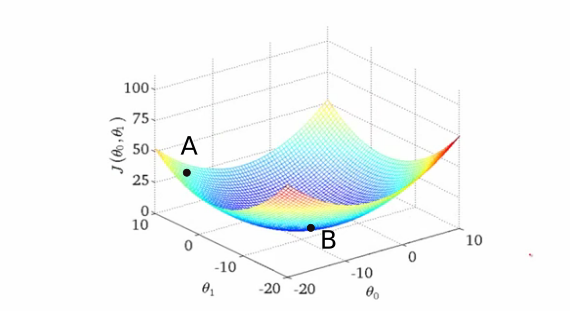
\includegraphics[width=0.8\textwidth]{Figures/gd.png}
	\caption{Estructura de la imagen de entrada \\ Fuente:  \href{https://blog.paperspace.com/intro-to-optimization-in-deep-learning-gradient-descent/}{\textit{https://blog.paperspace.com/}}}
	\label{image}
\end{figure} 

Dentro de la gradiente de descenso podemos diferenciar 3 variantes de acuerdo al la cantidad de datos que se usan para calcular la gradiente de nuestra función objetivo entre estas variantes tenemos a:\\

\subsubsection{Batch gradient descent}
Esta variante calcula la gradiente de descenso de una función de costo, con respecto a un parámetro $\theta$, \textit{para todo el conjunto de datos}. En la ecuación 4.1 podemos observar la actualización que se dará para cada ejecución. $\eta$ representa la tasa o tamaño de los pasos para encontrar el mínimo local.
\begin{equation}
\label{bgds}
\begin{aligned}
\theta &= \theta - \eta \nabla_{\theta} J(\theta)
\end{aligned}
\end{equation}
La ecuación 4.1 asegura la convergencia para mínimo global en una superficie convexa y mínimo local para una superficie no convexa. Entre las dificultades de este método tenemos que puede llegar a ser lento y que esta limitado por la cantidad de datos, ya que esta puede superar a la memoria nuestro computador.	
\subsubsection{Stochastic gradient descent}
Otra variante es \textit{Stochastic gradient descent} que a diferencia del método anterior, realiza las actualizaciones para cada ejemplo de entrenamiento de $(x^{i},y^{i})$ de esta forma se evitan problemas como la generación de redundancia debido a que se realiza una actualización por cada ejemplo de entrenamiento.
\begin{equation}
\label{sgds}
\begin{aligned}
\theta &= \theta - \eta \nabla_{\theta} J(\theta,x^{i},y^{i})
\end{aligned}
\end{equation}
En la figura 4.4 vemos que la función de costo usando SGD fluctúa demasiado esto podría representar un problema pero por el contrario, esta figura representa que el método SGD es capaz de saltar de un mínimo local a otro. Esto permite encontrar mínimos locales potencialmente mejores.

\begin{figure}[H]
	\centering
	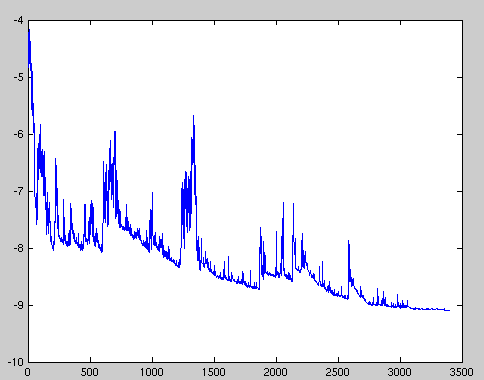
\includegraphics[width=0.5\textwidth]{Figures/sgd.png}
	\caption{Función costo en SGD \\ Fuente:  \href{https://www.doc.ic.ac.uk/~js4416/163/website/neural-networks/optimisers.html}{\textit{www.doc.ic.ac.uk}}}
	\label{funcion costo}
\end{figure} 

\subsubsection{Mini-batch gradient descent}
Este método pude verse como una mezcla de los 2 métodos anteriores, en lugar de aplicarlo para un conjunto entero de datos, los datos se dividen en pequeños conjuntos o mini batches, estos conjunto alimentan nuestro modelo de nuestra red.\\			
Este método nos permite reducir la varianza de las actualizaciones de los parámetros lo cual nos permite una convergencia más estable. El tamaño de los mini-batches oscilan entre 50-250 y varían de acuerdo a su aplicación.

\begin{equation}
\label{mbgds}
\begin{aligned}
\theta &= \theta - \eta \nabla_{\theta} J(\theta,x^{i:i+n},y^{i:i+n})
\end{aligned}
\end{equation}

Mini-batch gradient descent es necesario elegir un $\nabla$ adecuado. Debido  que uno pequeño puede ocasionar una convergencia lenta y una grande puede ocasionar que la fluctué entre los valores mínimos y no converga.\\
Una de sus ventajas principales es que aprovecha el rendimiento de las GPUs para realizar cálculos más rápidos, esto se debe a que la información se guarda como tensores(Matrices de gran dimensión) y las GPUs realizan cálculos de operaciones de matrices más rápidos que una CPU. Es común encontrar a este en otras lecturas como \textit{Stochastic gradient descent} sin realizar distinción alguna del método anteriormente descrito.

\subsection{Optimizadores}
En esta sección analizaremos y entenderemos como funcionan algunos optimizadores en el proceso de mejorar la convergencia de la gradiente de descenso.
\subsubsection{Momentum}
Las SGD tienen problemas para desplazarse en áreas con donde la superficie se curva más en una dimensión que en otra, estos lugares son los alrededores de los óptimos locales. En este escenario la SGD oscilará en la curvatura y descenderá lentamente hacia el óptimo como se muestra en la figura 4.5.
\begin{figure}[H]
	\centering
	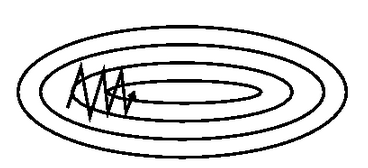
\includegraphics[width=0.5\textwidth]{Figures/momentum1.png}
	\caption{Actualización sin momentum \\ Fuente:  \href{https://www.doc.ic.ac.uk/~js4416/163/website/neural-networks/optimisers.html}{\textit{www.doc.ic.ac.uk}}}
	\label{momentum1}
\end{figure}
El momentum es un método que ayuda a la SGD a acelerar en la dirección correcta, mientras evitas las oscilaciones. El momentum lográ esto añadiendo una fracción $\gamma$ del vector de actualización pasado a nuestro vector presente tal como se muestra en las ecuaciones 4.4.\\ Un valor comúnmente elegido es $\gamma =0.9 $, en las actualización el valor del momentum aumenta para dimensiones cuyos gradientes apuntan en la misma dirección y disminuye para dimensiones en la que la gradiente cambia de dirección. Esto nos asegura que tendremos una convergencia más rápida con una oscilación reducida.En la figura 4.6 se observa gráficamente la aceleración de la convergencia en la SGD.

\begin{equation}
\label{mbgds}
\begin{aligned}
\nu_{t}&=\gamma \nu_{t-1} +  \eta \nabla_{\theta} J(\theta)\\
\theta &= \theta -\nu_{t}
\end{aligned}
\end{equation}

\begin{figure}[H]
	\centering
	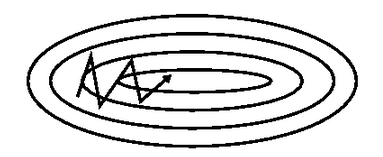
\includegraphics[width=0.5\textwidth]{Figures/momentum2.png}
	\caption{Actualización con momentum \\ Fuente:  \href{https://www.doc.ic.ac.uk/~js4416/163/website/neural-networks/optimisers.html}{\textit{www.doc.ic.ac.uk}}}
	\label{momentum2 }
\end{figure}

\subsubsection{Nesterov accelerated gradient (NAG)}
Este método permite que nuestro descenso sea más controlado, ya que reduce la velocidad antes de volver a subir una pendiente en nuestra superficie de la función de costo. Esta técnica es una variante de momentum donde se usa el término $\gamma \nu_{t-1}$ para mover los parámetros de $\theta$. Al calcular el valor de $\theta - \gamma \nu_{t-1}$ nos permite tener una aproximación de donde se encontrá la siguiente posición de los parámetros. Por lo tanto no calculamos la gradiente en el parámetro $\theta$ actual sino que se calcula en una posición futura aproximada.




\begin{equation}
\label{mbgds}
\begin{aligned}
\nu_{t}&=\gamma \nu_{t-1} + \eta \nabla_{\theta} J(\theta- \gamma \nu_{t-1})\\
\theta &= \theta -\nu_{t}
\end{aligned}
\end{equation}

En la figura 4.7 observamos el proceso. Primero el momentum calcula la gradiente actual(vector azul pequeño)  y luego da un gran salto en la dirección de la gradiente actualizada acumulada (gran vector azul), el NAG primero realiza un gran salto en dirección del gradiente acumulado previo(vector marrón), luego realiza un corrección(vector rojo), esto nos da como resultado la actualización completa de NAG(vector verde). Este calculo anticipado es muy importante debido a que nos impide ir demasiado rápido y mejora la capacidad de respuesta lo cual aumenta el rendimiento de las CNN.
\begin{figure}[H]
	\centering
	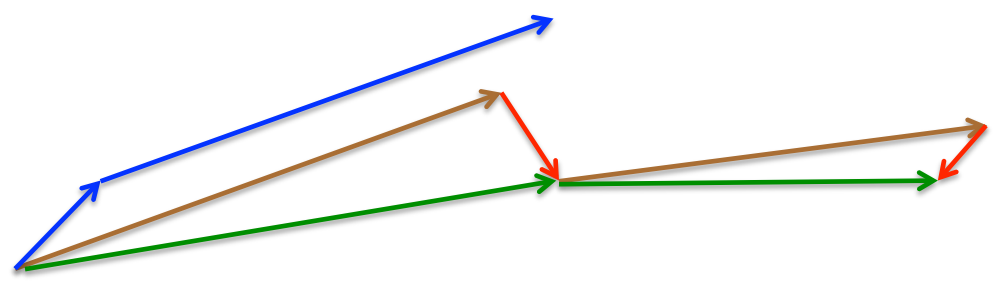
\includegraphics[width=0.5\textwidth]{Figures/nesterov.png}
	\caption{Convergencia Nesterov\\ Fuente:  \href{https://www.doc.ic.ac.uk/~js4416/163/website/neural-networks/optimisers.html}{\textit{www.doc.ic.ac.uk}}}
	\label{nesterov }
\end{figure}
\subsubsection{Adagrad}
Es un algoritmo optimización basado en la gradiente de descenso, este adapta la tasa de aprendizaje. A este tipo de método se les conoce como \textit{adaptativos}. Adagrad realiza actualizaciones más pequeñas para parámetros con características que se repiten con más frecuencia y una tasa alta  para parámetros con características pocas frecuentes. Este método mejor en gran forma nuestra SGD, entre sus ventajas tenemos que es usado para entrenar redes neuronales a gran escala.


En métodos anteriores se usaba la actualización de todos los parámetros $\theta$ al mismo tiempo esto debido a que se usaba la misma tasa de aprendizaje $\eta $. Adagrad usa una tasa de aprendizaje diferente para cada parámetro $\theta_{i}$ en cada paso de tiempo $t$.
En la ecuación 4.6 mostramos los cálculos de la gradiente en un tiempo t.
\begin{equation}
\label{adagrad1}
\begin{aligned}
g_{t,i}&=\nabla_{\theta} J(\theta_{t,i})\\
\theta_{t+1,i} &= \theta_{t,i} -\eta \cdot g_{t,i}
\end{aligned}
\end{equation}
El termino $\cdot g_{t,i}$ representa el valor de la gradiente en el paso de tiempo $t$, el cual es la derivada de la función objetivo con respecto al termino $\theta_{i}$.

Adagrad modifica la idea de utilizar una tasa $\eta$ fija, podemos observar el la ecuación 4.7 es una variante de la ecuación 4.6. En donde se modifica la tasa de aprendizaje en cada paso de tiempo $t$ para todos los parámetros $\theta_{i} $ basándonos en los valores de las gradientes pasadas que fueron calculas para $\theta_{i}$
\begin{equation}
\label{adagrad2}
\begin{aligned}
\theta_{t+1,i} &= \theta_{t,i} - \frac{\eta}{\sqrt{G_{t,ii}+\epsilon}} \cdot g_{t,i}
\end{aligned}
\end{equation}

\begin{itemize}
	\item $G_{t,ii}$: representa la suma de los cuadrados de las gradientes pasadas con respecto a $\theta_{i}$
	\item $\epsilon $ es un término pequeño para evitar la división por 0. $\epsilon$ encuentra en el orden de $10^{-8}$.
\end{itemize}
Como $G_{t} \in \Re^{dxd} $contiene la suma de los cuadrados de las gradientes pasados con respecto a todos los parámetros de $\theta$ a lo largo de la diagonal de su matriz. Esto permite que se pueda realizar el producto matriz-vector.
\begin{equation}
\label{adagrad3}
\begin{aligned}
\theta_{t+1,i} &= \theta_{t,i} - \frac{\eta}{\sqrt{G_{t}+\epsilon}} \odot g_{t,i}
\end{aligned}
\end{equation}
El método Adagrap en palabras de sus autores:
\textquotedblleft Informalmente nuestros procedimientos dan a las características más frecuentes tasas de aprendizaje bajas y para características poco frecuentes tasas de aprendizaje altas. Por lo tanto, la adaptación permite identificar características predictivas pero comparativamente raras. \textquoteright  \cite{ADA} 

De esta afirmación notamos que el principal beneficio de Adagrad es que nos evita el hecho de trabajar con una tasa fija por otro lado su principal desventaja se basa en el la suma de los gradientes al cuadrado aumentará en cada iteración lo cual provocará que su tasa sea cada vez más pequeña.


\subsubsection{RMSprop}
Es un método de aprendizaje por adaptación de la tasa que fue propuesto por Geoff Hinton.
Este modelo se desarrollo con el objetivo resolver el problema de disminuir radicalmente la tasa de aprendizaje en Adagrad.\\ RMSprop divide la tasa de aprendizaje mediante el decaimiento del promedio de la suma de las gradientes al cuadrado.
\begin{equation}
\label{RMS}
\begin{aligned}
E[g^2]_{t} &= \gamma E[g^2]_{t-1} + (1-\gamma)g^{2}_{t}\\
\theta_{t+1} &= \theta_{t} - \frac{\eta}{\sqrt{E[g^2]_{t} +\epsilon }} g_{t}
\end{aligned}
\end{equation}
\begin{itemize}
	\item $E[g^2]$: Promedio de la raíz de nuestro gradiente en cada peso.
	\item $\gamma$  : Parámetro de decaimiento
	\item $\eta$    : Tasa de aprendizaje
\end{itemize}
Divide la gradiente $g_{t}$ por la raíz $\sqrt{E[g^2]_{t} +\epsilon}$ hace que el aprendizaje trabaje mucho mejor.
\subsubsection{Adam	}
Adam es un algoritmo de optimización que desarrollado por Diederik Kingma y Jimmy ba\cite{ADAM} .
Adaptative moment estimation  o Adam, calcula una tasa de aprendizaje adaptativo para cada parámetro. Este método mantiene un decaimiento exponencial del promedio de las gradientes anteriores. El método tiene refiere los mínimos en las superficies de error.
 En la ecuación 4.10 mostramos el cálculo del promedio de decaimiento de las gradientes pasadas $m_{t}$ y el cuadrado de las gradientes pasadas $v_{t}$
\begin{equation}
\label{adam1}
\begin{aligned}
m_{t} &= \beta_{1} m_{t-1} +(1-\beta_{1})g_{t} \\
v_{t} &= \beta_{2} v_{t-1} +(1-\beta_{2})g_{t}^2
\end{aligned}
\end{equation}

\begin{itemize}
	\item $m_{t}:$ Primer momento (media)
	\item $v_{t}:$ Segundo momento de la gradiente
	\item $\beta_{1}:$ Taza de decaimiento del primer momento.
	\item $\beta_{2}:$ Taza de decaimiento del segundo momento.
\end{itemize}
En la ecuación 4.11 mostramos la forma de calcular estimado de la primer y segundo momento.
\begin{equation}
\label{adam2}
\begin{aligned}
\hat{m_{t}}&= \frac{m_{t}}{1-\beta_{1}^{t}} \\
\hat{v_{t}} &= \frac{v_{t}}{1-\beta_{2}^{t}}
\end{aligned}
\end{equation}

\begin{itemize}
	\item $\hat{m_{t}}:$ Estimación del Primer momento (media)
	\item $\hat{v_{t}}:$ Estimación del Segundo momento de la gradiente.
\end{itemize}

La ecuación 4.12 muestra la regla de actualización en Adam. Se utiliza el $\epsilon$ para prevenir una división por cero.
\begin{equation}
\label{adam3}
\begin{aligned}
\theta_{t+1}&= \theta_{t+1} - \frac{\eta}{\sqrt{\hat{v_{t}}}+\epsilon} \hat{m_{t}}	
\end{aligned}
\end{equation}


%\newpage
$\ $
%\thispagestyle{empty} % para que no se numere esta pagina
\chapter{Conclusiones y Trabajo Futuro}
ESTE CAPÍTULO ES UNO DE LOS MÁS IMPORTANTES, POR NO DECIR EL QUE MÁS. EN ÉL, EL JURADO VA A TENER CLARO QUÉ HA APRENDIDO EL ALUMNO Y CÓMO LO HA DESARROLLADO, LOS PROBLEMAS QUE HAN SURGIDO Y COMO LOS HA SOLUCIONADO...
ADEMÁS DE QUE EL ALUMNO DEJARÁ CLARO QUE SE HA ESPECIALIZADO EN LA TEMÁTICA Y DEJARÁ EN ESCRITO TODO LO APRENDIDO Y COMO CONTINUARÁ CON LA TEMÁTICA EN POSTERIORES ESTUDIOS DEL MISMO TEMA

\section{Conclusiones}


\begin{itemize}

\item[•] CONCLUSION 1: ASDFASDFASDFAS.
\item[•] CONCLUSION 2: ASDFASDFASDFAS. 

\end{itemize}
Además de lo anterior ....

\section{Trabajo Futuro}
COMO SE VA A SEGUIR TRABAJANDO CON ESTA TEMÁTICA Y QUE FALTA POR DESARROLLAR. ADEMÁS SE ACONSEJARÁ SEGUIR UNA METODOLOGÍA PARA QUE LAS PERSONAS QUE QUIERAN SEGUIR TRABAJANDO ESTA TEMÁTICA

\subsection*{NASDFASDFASF}
ADFASDFASDFA

\subsection*{NASDFASDFASF}
ADFASDFASDFA

\subsection*{NASDFASDFASF}
ADFASDFASDFA

%\afterpage{\blankpage}
\chapter{Conclusiones y Trabajo Futuro}
En este capítulo se describirán las conclusiones generales que se encontraron al probar y estudiar los distintos métodos de optimización utilizados para el proceso de acelerar el entrenamiento de una red neuronal convolucional.\\ Además, se propondrán algunas mejoras para que el trabajo obtenga mejores resultados.


\section{Conclusiones}


\begin{itemize}

\item[•] Los métodos de optimización Adam y RMSprop obtuvieron los mejores resultados de precisión en ambas pruebas.
\item[•] A pesar de que el método de optimización Adam fue propuesto a partir del RMSprop. Adam fue superado en las pruebas realizadas.
\item[•] El método Adagrad fue el que menor precisión obtuvo en las pruebas, esto se debió a su dificultad de trabajar con la suma de las gradientes al cuadrado lo cual poco a poco redujo su taza de aprendizaje.
\item[•] El RMSprop como una mejora del Adagrad, obtuvó mejores resultados que el Adagrad. Esto debido a que trabajo con el promedio de la raíz de la gradiente anterior y tasas de decaimiento para controlar el problema de la disminución de la tasa de aprendizaje del método Adagrad.

\end{itemize}


\section{Trabajo Futuro}
El propósito general de este seminario I fue adquirir el conocimiento y experiencia necesarios para poder trabajar con redes neuronales profundas. Los métodos de optimización fueron una manera de introducirme al área de las redes convolucionales y comprender las ventajas y desventajas de algunos métodos. \\
Los temas de aprendizaje automático y en particular del aprendizaje profundo son muy amplios y en este seminario se trato de acoplar los temas pero no se realizó un análisis más detallado debido a la amplitud del área. \\
En el Seminario II se trabajará con más detalle el campo de redes neuronales convolucionales, además se tratará de diseñar un red neuronal convolucional y comparar este modelo con algunos actualmente usados. Además de realizar un implementación más interactiva .\\ Este seminario fue limitado debido a la capacidad de la tarjeta gráfica usada ya que en algunos ensayos la memoria era insuficiente para el futuro seminario se planea realizar las pruebas en mejores equipos como por ejemplo contratar servicios de máquinas virtuales de Amazon u otro proveedor.



%\afterpage{\blankpage}\textsl{}
\bibliography{main}
\bibliographystyle{unsrt}
\afterpage{\blankpage}
\appendix
% Appendix A

\chapter{Arquitectura de la red y Resultados obtenidos} % Main appendix title

\label{AppendA} % For referencing this appendix elsewhere, use \ref{AppendixA}
\section{Capas de la red neuronal convolucional}

\begin{figure}[H]
		\begin{center}
		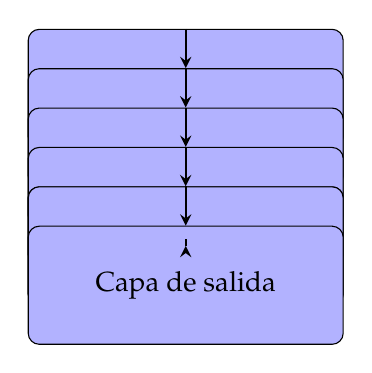
\begin{tikzpicture}[node distance=0.5cm]
		\node (input) [startstop] {Capa de Entrada};
		\node (conv1) [startstop, below of=input] {Capa de convolución 1};
		
		\node (pool1) [startstop, below of=conv1] {Capa Pooling 1};
		\node (conv2) [startstop, below of=pool1] {Capa de convolución 2};
		\node (pool2) [startstop, below of=conv2] {Capa Pooling 2};
		\node (full) [startstop, below of=conv2] {Full Layer};
		\node (exit) [startstop, below of=full] {Capa de salida};
		\draw [arrow] (input) -- (conv1) ;
		\draw [arrow] (conv1) -- (pool1);
		\draw [arrow] (pool1) -- (conv2);
		\draw [arrow] (conv2) -- (pool2);
		\draw [arrow] (pool2) -- (full);
		\draw [arrow] (full) -- (exit);
		\end{tikzpicture}
	\end{center}
	\caption{Capas de la red neuronal usada \\ Fuente:  \textit{Fuente Propia}}
\end{figure}



\section{Resultados de precisión de entrenamiento}
\subsection{CIFAR-10}
\begin{figure}[H]
	\begin{centering}
		\subfloat[fig 1]{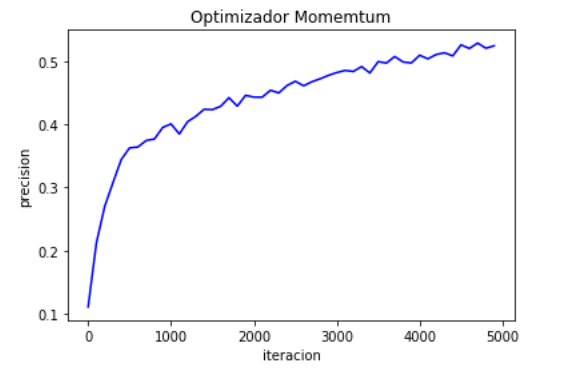
\includegraphics[width=0.45\textwidth]{Figures/momemtum5000.png}} 
		\subfloat[fig 2]{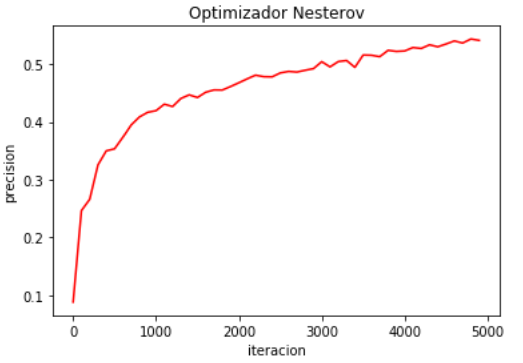
\includegraphics[width=0.45\textwidth]{Figures/nesterov5000.png}}\\
		\subfloat[fig 3]{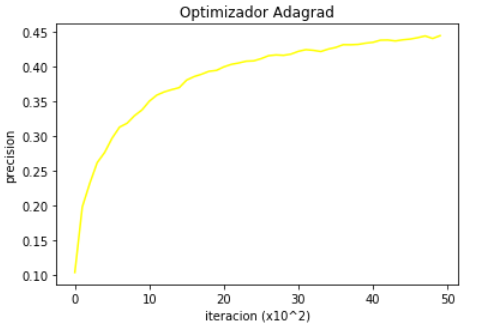
\includegraphics[width=0.45\textwidth]{Figures/adagrad5000.png}}
		\subfloat[fig 3]{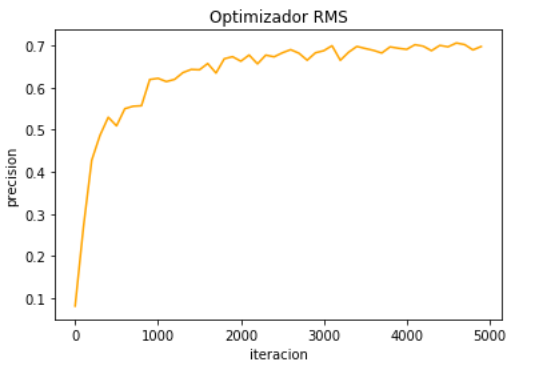
\includegraphics[width=0.45\textwidth]{Figures/rms5000.png}}\\
		\subfloat[fig 4]{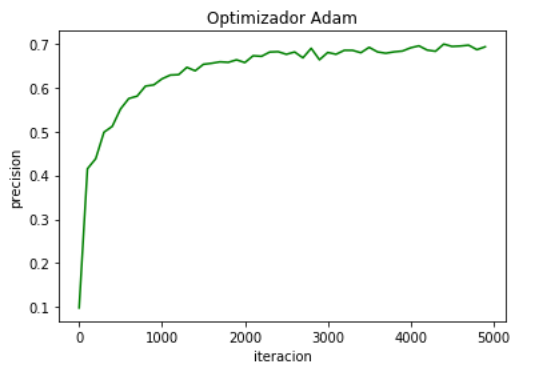
\includegraphics[width=0.5\textwidth]{Figures/adam5000.png}} 
		\caption{optmizadores 5000 epochs \\ Fuente :{\textit{Fuente Propia}}}
		\label{some example0}
	\end{centering}

\end{figure}


\begin{figure}[H]
	\begin{centering}
		\subfloat[fig 1]{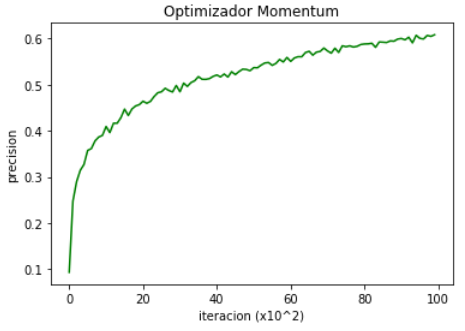
\includegraphics[width=0.55\textwidth]{Figures/momemtum10000.png}} 
		\subfloat[fig 2]{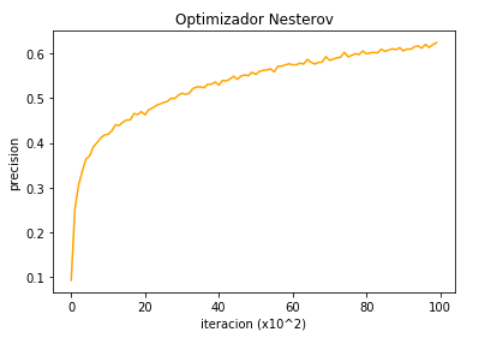
\includegraphics[width=0.55\textwidth]{Figures/nesterov10000.png}}\\
		\subfloat[fig 3]{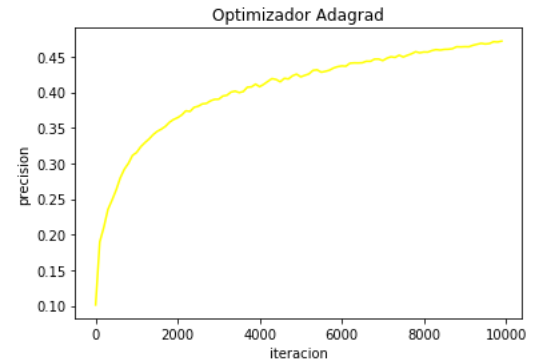
\includegraphics[width=0.55\textwidth]{Figures/adagrad10000.png}}
		\subfloat[fig 3]{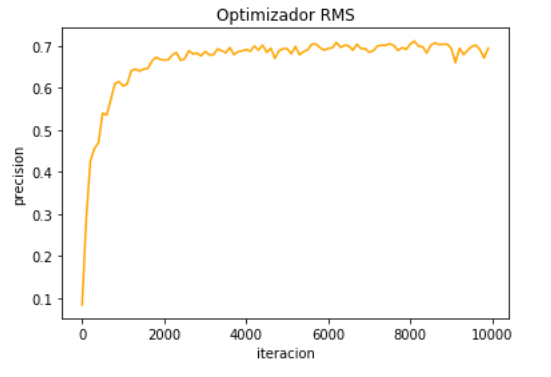
\includegraphics[width=0.55\textwidth]{Figures/rms10000.png}}\\
		\subfloat[fig 4]{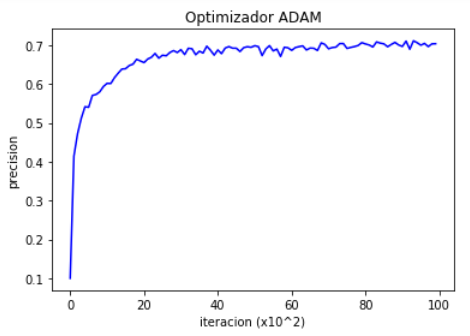
\includegraphics[width=0.6\textwidth]{Figures/adam10000.png}} 
		\caption{optmizadores 10000 epochs\\ Fuente:  \textit{Fuente Propia}}
		\label{some example1}
	\end{centering}
	
\end{figure}

\begin{figure}[H]
	\begin{centering}
		\subfloat[fig 1]{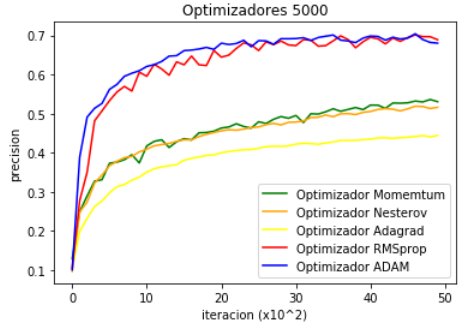
\includegraphics[width=0.8\textwidth]{Figures/optimizadores5000.png}} 
		\caption{Comparación de precisión de optimizadores para 5000 epochs\\ Fuente:  \textit{Fuente Propia}}
		\label{some example2}
	\end{centering}
	
\end{figure}

\begin{figure}[H]
	\begin{centering}
		\subfloat[fig 1]{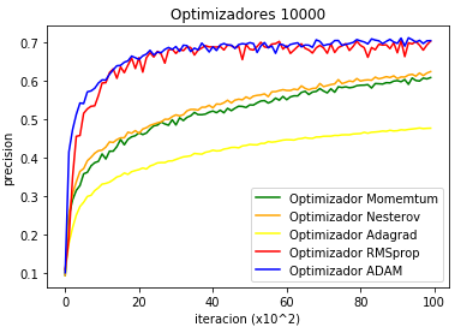
\includegraphics[width=0.8\textwidth]{Figures/optimizadores10000.png}} 
		\caption{Comparación de optimizadores para 10000 epochs\\ Fuente:  \textit{Fuente Propia}}
		\label{some example3}
	\end{centering}
	
\end{figure}

\subsection{CIFAR-100}

\begin{figure}[H]
	\begin{centering}
		\subfloat[fig 1]{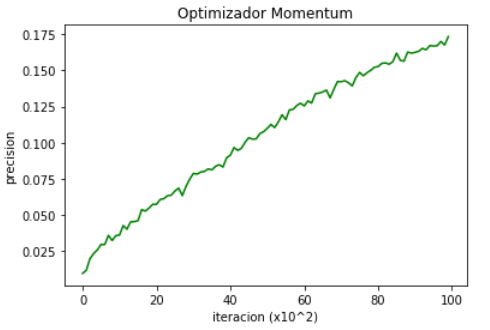
\includegraphics[width=0.55\textwidth]{Figures/100momemtum10000.png}} 
		\subfloat[fig 2]{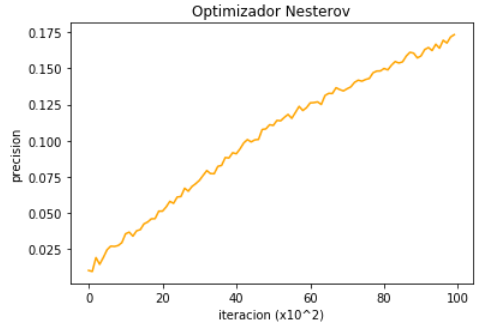
\includegraphics[width=0.55\textwidth]{Figures/100nesterov10000.png}}\\
		\subfloat[fig 3]{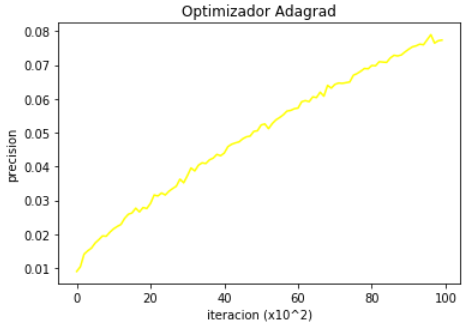
\includegraphics[width=0.55\textwidth]{Figures/100adagrad10000.png}}
		\subfloat[fig 3]{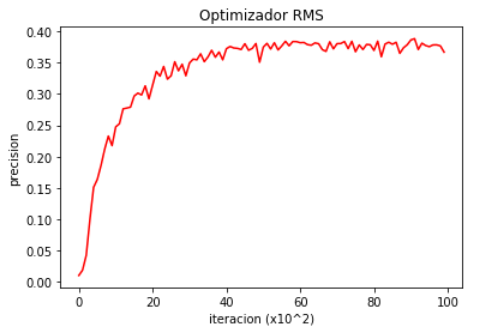
\includegraphics[width=0.55\textwidth]{Figures/100rms10000.png}}\\
		\subfloat[fig 4]{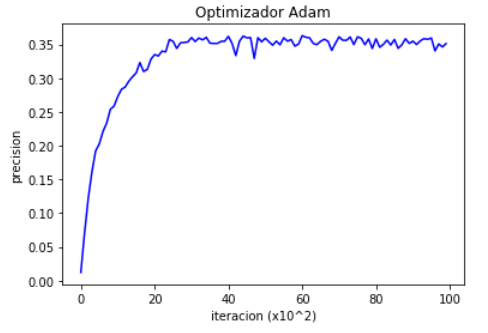
\includegraphics[width=0.6\textwidth]{Figures/100adam10000.png}} 
		\caption{optmizadores 10000 epochs\\ Fuente:  \textit{Fuente Propia}}
		\label{some exampleasa1}
	\end{centering}
	
\end{figure}



\begin{figure}[H]
	\begin{centering}
		\subfloat[fig 1]{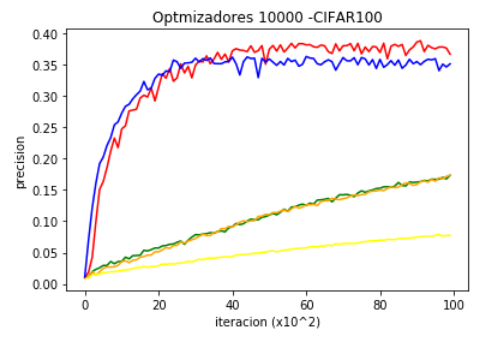
\includegraphics[width=0.8\textwidth]{Figures/cifar100result.png}} 
		\caption{Comparación de optimizadores para 10000 epochs - CIFAR100\\ Fuente:  \textit{Fuente Propia}}
		\label{some example32}
	\end{centering}
	
\end{figure}
\section{Resultados del error en el entrenamiento}
\subsection{CIFAR-10}
\begin{figure}[H]
	\begin{centering}
		\subfloat[fig 1]{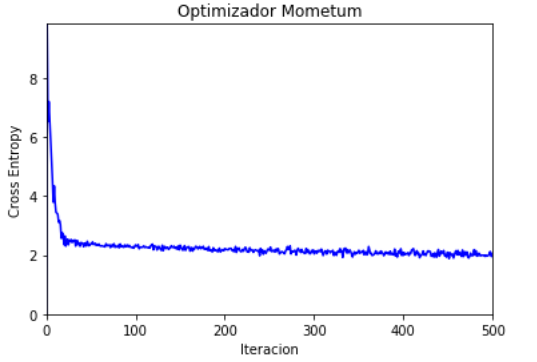
\includegraphics[width=0.5\textwidth]{Figures/momemtumcross5000.png}} 
		\subfloat[fig 2]{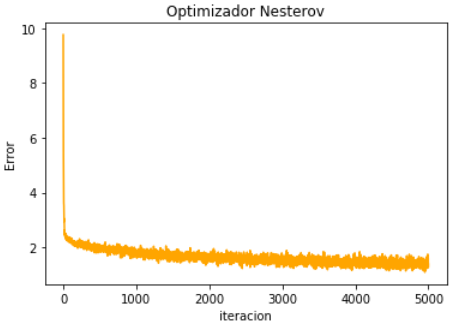
\includegraphics[width=0.5\textwidth]{Figures/nesterovcross5000.png}}\\
		\subfloat[fig 3]{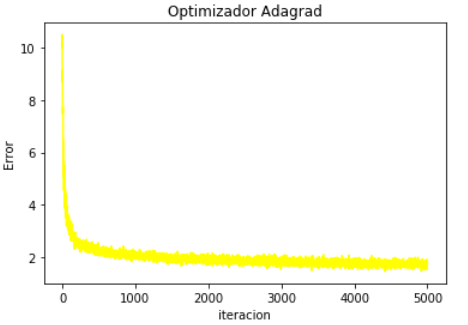
\includegraphics[width=0.5\textwidth]{Figures/adagradcross5000.png}}
		\subfloat[fig 3]{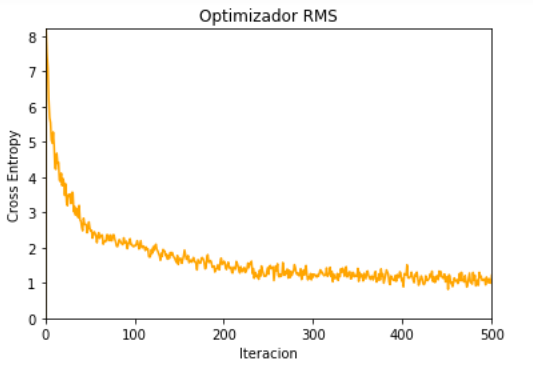
\includegraphics[width=0.5\textwidth]{Figures/rmscross5000.png}}\\
		\subfloat[fig 4]{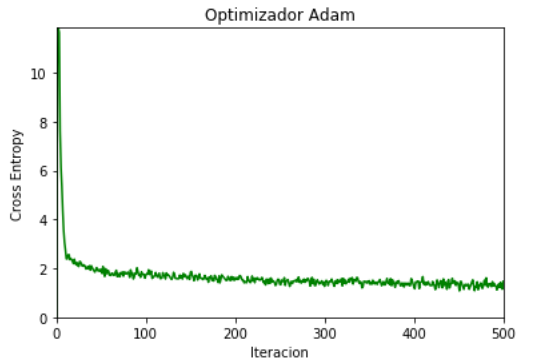
\includegraphics[width=0.5\textwidth]{Figures/adamcross5000.png}} 
		\caption{Error en los optimizadores 5000 epochs\\ Fuente:  \textit{Fuente Propia}}
		\label{some}
	\end{centering}
	
\end{figure}

\begin{figure}[H]
	\begin{centering}
		\subfloat[fig 1]{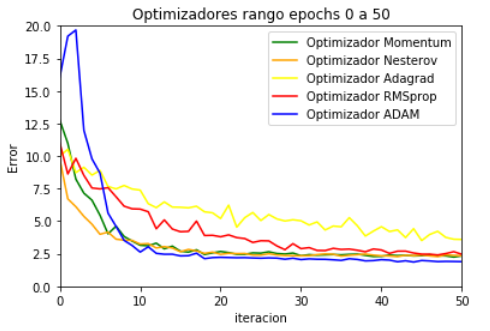
\includegraphics[width=0.8\textwidth]{Figures/optimizadorescross5000050}} 
		\caption{Comparación de las funciones de costo rango 0-50\\ Fuente:  \textit{Fuente Propia}}
		\label{some example5}
	\end{centering}
	
\end{figure}

\begin{figure}[H]
	\begin{centering}
		\subfloat[fig 1]{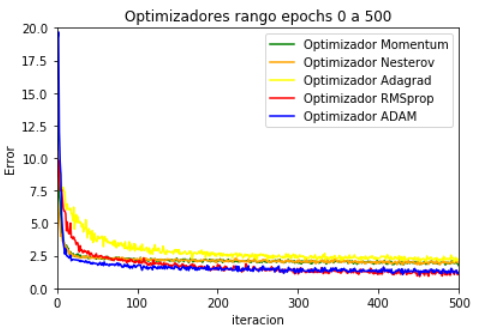
\includegraphics[width=0.8\textwidth]{Figures/optimizadorescross50000500}} 
		\caption{Comparación de las errores rango 0-500\\ Fuente:  \textit{Fuente Propia}}
		\label{some example6}
	\end{centering}
	
\end{figure}
\begin{figure}[H]
	\begin{centering}
		\subfloat[fig 1]{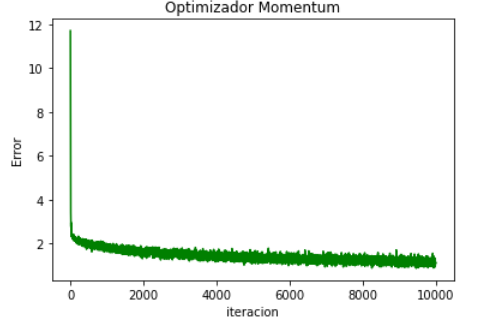
\includegraphics[width=0.6\textwidth]{Figures/momemtumcross10000.png}} 
		\subfloat[fig 2]{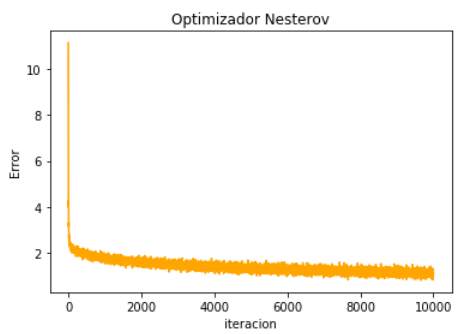
\includegraphics[width=0.6\textwidth]{Figures/nesterovcross10000.png}}\\
		\subfloat[fig 3]{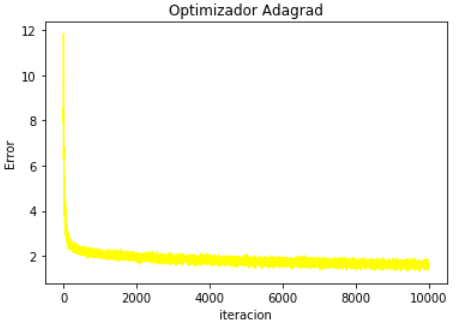
\includegraphics[width=0.6\textwidth]{Figures/adagradcross10000.png}}
		\subfloat[fig 3]{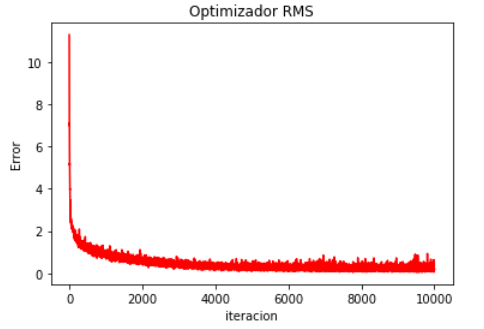
\includegraphics[width=0.6\textwidth]{Figures/RMScross10000.png}}\\
		\subfloat[fig 4]{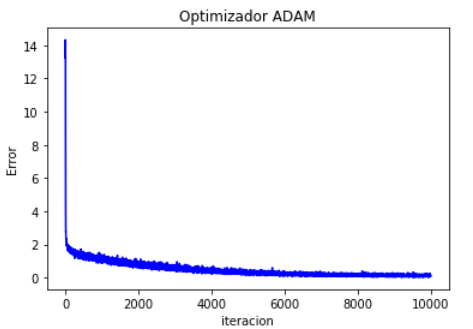
\includegraphics[width=0.6\textwidth]{Figures/adamcross10000.png}} 
		\caption{Error en los optimizadores 10000 epochs -CIFAR10\\ Fuente:  \textit{Fuente Propia}}

	\end{centering}
	
\end{figure}

\subsection{CIFAR-100}
\begin{figure}[H]
	\begin{centering}
		\subfloat[fig 1]{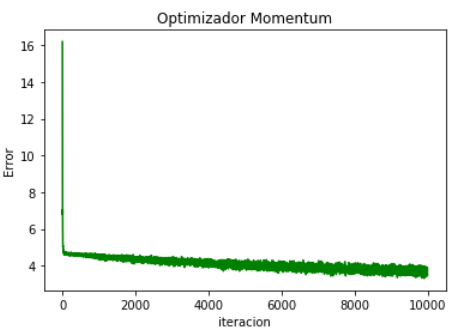
\includegraphics[width=0.6\textwidth]{Figures/100momentumcross10000.png}} 
		\subfloat[fig 2]{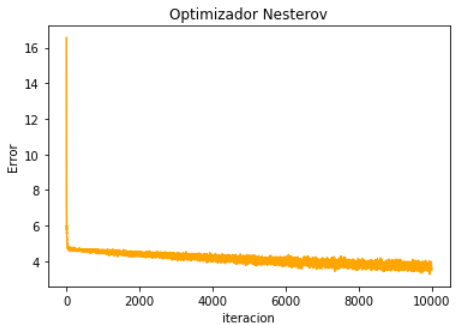
\includegraphics[width=0.6\textwidth]{Figures/100nesterovcross10000.png}}\\
		\subfloat[fig 3]{\includegraphics[width=0.6\textwidth]{Figures/100adagradcross10000.png}}
		\subfloat[fig 3]{\includegraphics[width=0.6\textwidth]{Figures/100rmscross10000.png}}\\
		\subfloat[fig 4]{\includegraphics[width=0.6\textwidth]{Figures/100adamcross10000.png}} 
		\caption{Error en los optimizadores con 10000 epochs - CIFAR 100 \\ Fuente:  \textit{Fuente Propia}}
		\label{some2341}
	\end{centering}
	
\end{figure}

\begin{figure}[H]
	\begin{centering}
		\subfloat[fig 1]{\includegraphics[width=0.8\textwidth]{Figures/cifar100error.png}} 
		\caption{Comparación los errores rango 9900-10000\\ Fuente:  \textit{Fuente Propia}}
		\label{COMPARACION}
	\end{centering}
	
\end{figure}


\end{document}